\chapter{Related Works}  \label{ch:review}

In this chapter, I select the most outstanding studies based on a self-defined criteria (either published in a set of pre-selected venues or performed the highest impact by receiving at least fifty citations). To better introduce these papers in a well-organized manner, I categorize them into five following tracks borrowing ideas from aforementioned survey studies \cite{fortunato2010community, fortunato2016community, coscia2011classification}. In detail, papers in the Graph Type track focus on detecting communities in different types of graphs, such as heterogeneous or sparse graphs. In the Task track, the selected studies aim to solve particular tasks in community detection, such as deciding the correct number of communities. In the Methodological track, the introduced studies solve the general community detection problem via different types of model frameworks such as Modularity or spectral methods. In the Application track, selected studies discuss community detection applications and how to apply them to other disciplines. In the last Evaluation track, it lists papers to summarize the evaluation metrics widely used for model justification and comparison. 


\section{Graph Types}
Graph types are various and complex. Different type of graphs have their particular characteristics, which requires to be handled by special techniques. With the rapid development of graph mining, more and more complex graphs are constructed from real scenarios and analyzed by researchers, which offers the possibility to summarize several main types and relevant works in this section. Particularly, the following paragraphs introduce five main types of graph which are most frequently appeared in research studies and tightly connected with real-world scenarios, including heterogeneous \& multi-layer graph, sparse graph, dynamic graph, large graph and attribute graph. 

\subsection{Heterogeneous \& Multi-layer Graph} 

The research works about heterogeneous and multi-layer graph community detection are summarized together. The reason is that both types of graphs share very similar structure but still keep their own characteristics. For a heterogeneous graph, it should contains more than one type of node or edges. While for a multi-layer graph, it is composed from multiple single layer graphs. A single layer graph is with only one type of node/edge.  By connecting nodes across single layer graphs with edges, it formulates a multi-layer graph in the end. Figure \ref{fig:c2_hetero} clearly shows the definition difference between heterogeneous graph and multi-layer graph. In fact, multi-layer graph can be regarded as a particular type of heterogeneous graph. 

\begin{figure}
	% \setlength{\belowcaptionskip}{-10pt}
	\center
	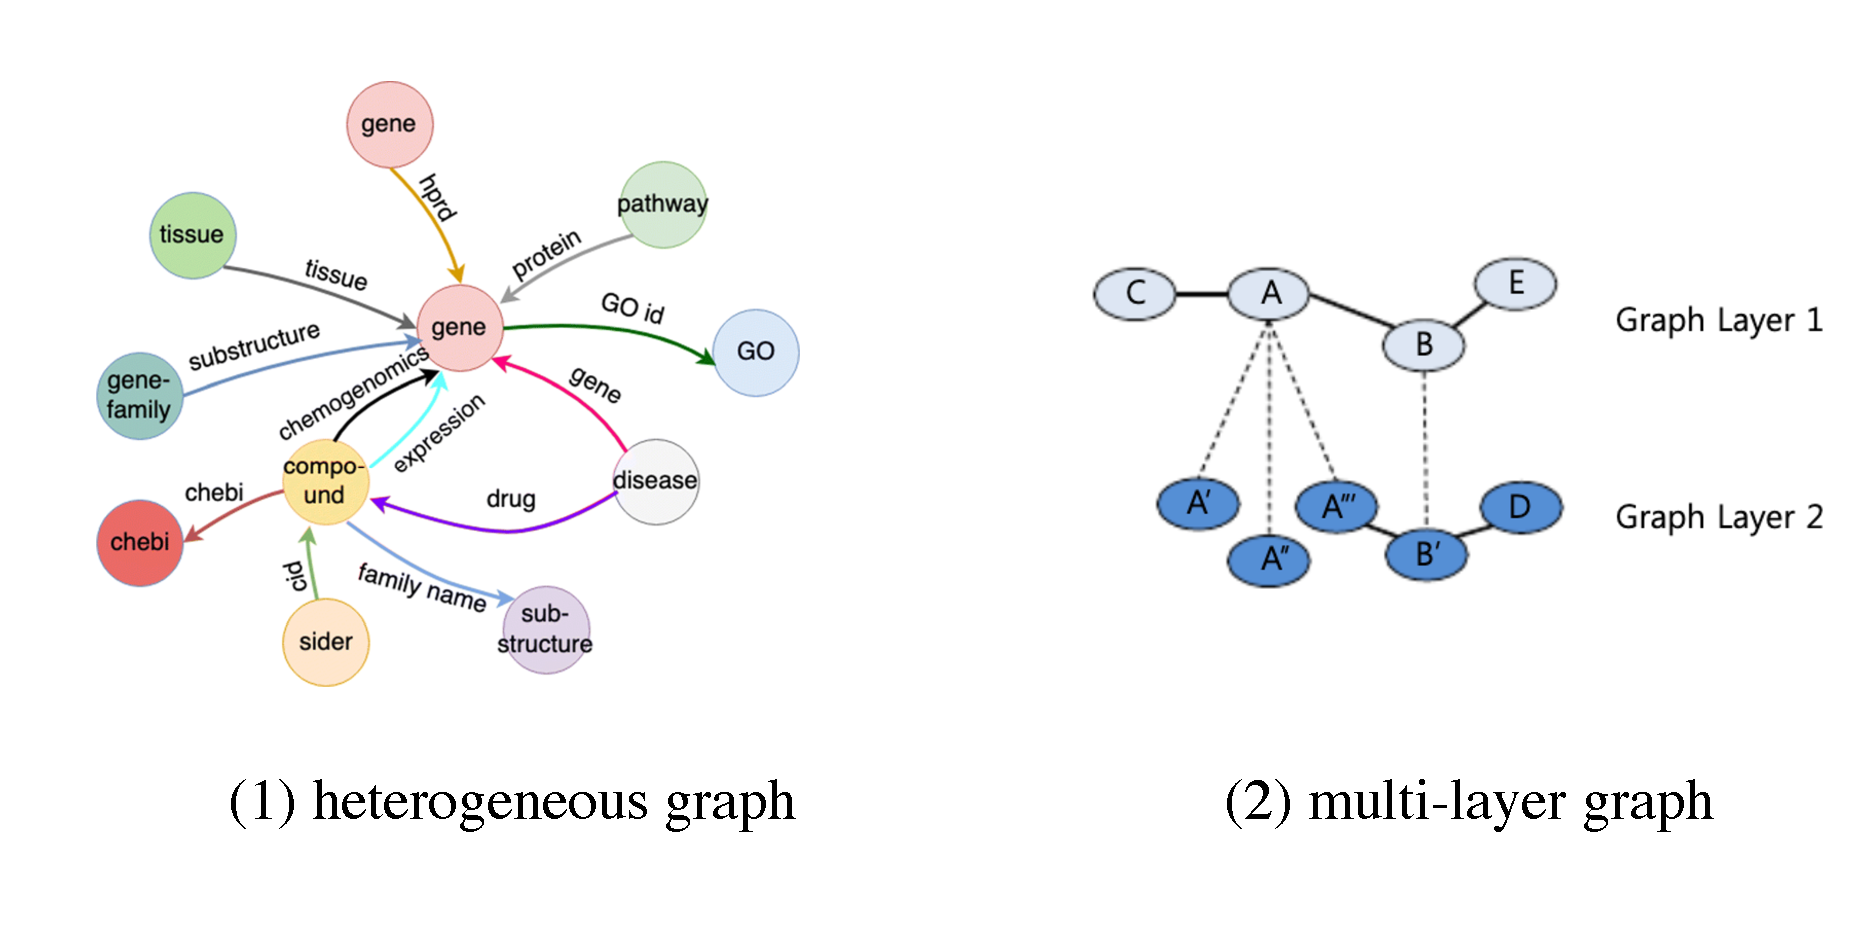
\includegraphics[width=\columnwidth]{img/chapter2/heterogenous.pdf} 
	\caption{Figure in the left is a typical heterogeneous medical graph in which nodes and edges refer to medical entities and their binding relationships from \cite{gao2019edge2vec}. Figure in the right is a multi-layer graph with two graph layers from \cite{kim2015community}.}
	\label{fig:c2_hetero}
\end{figure}  


Heterogeneous graph, also called heterogeneous information network, is a particularly complex graph which is ubiquitously appeared in current research works. By definition, a heterogeneous graph $G(V,E)$ has an extra node mapping function $\phi : V \rightarrow \mathcal{A}$ and an edge mapping function $\psi : E \rightarrow \mathcal{R} $ where each node $v \in V$ belongs to a particular node type $\phi(v) \in \mathcal{A}$ and each edge $e \in E$ belongs to a particular edge type $\psi(e) \in \mathcal{R}$. $\mathcal{A}$ is the collection of all node types and $\mathcal{R}$ is the collection of all edge types. A heterogeneous graph contains multiple node/edge types, which means at least either $|\mathcal{A}| > 1$ or $|\mathcal{R}| > 1$.

\cite{sun2013pathselclus} defines a graph structure called metapath, which is a path that connects node types with different types of edges and can be regarded as a general structure to represent path semantics. For example, a metapath in a scholarly graph can be ``Organization-(affiliated with)$\rightarrow$Author-(publish at)$\rightarrow$Venue'' where it contains three node types (``Organization'', ``Author'' and ``Venue'') and two types of edges (``affiliated with'' and ``publish at''). Particularly in this study, it integrates metapath selection with user guided clustering (a small set of nodes whose communities are known as prior information). In the end, it aims to learn the weights on selected metapaths to best satisfy the prior community knowledge via an EM approach.  

\cite{gupta2013community} introduces a joint approach to learn node affiliation distributions on popular communities in heterogeneous graph and detect node outliers which do not belong to any of the popular community distribution patterns in a holistic manner. It decomposes the heterogeneous graph into several homogeneous ones. The community detection step is derived from nonnegative matrix factorization framework and the refined outlier detection is learned via an iterative two-stage approach. In the NMF based community detection process, all prior-known community membership matrices of single node-type graphs $\{T_1,....,T_k\}$ can be used to calculate node community distribution under each node type:

\begin{equation}
	\argmin_{W,H}\sum_{i=1}^{k}||T_i - W_{i}H_{i}||^2 + \alpha \sum_{i \leq j \leq k}^{k}||H_i - H_j||^2
\end{equation}
which should subject to $W_i \geq 0$ and $H_i \geq 0$ for $ \forall i \leq k$. $W_i$ is the node vector representation matrix in the $i_{th}$ node-type graph and $H_i$ is the related community centroid matrix. The later part is the regularized term.

A node outlier score is calculated as the distance ($Dist(\cdot)$) between the current node community membership and its nearest community centroid:

\begin{equation}
S(i) =  \argmin_{j} Dist(T_{k_{(i,\cdot)}}, H_{k_{(j,\cdot)}})
\end{equation} 
Top $\rho$ nodes with largest outlier score will be regarded as outliers in current step. In an iterative learning process, the NMF method is optimized by reducing the detected outliers from the whole graph to support new node outlier detection. It stops when no outlier nodes are found out.

\cite{sun2012relation} solves a heterogeneous and incomplete graph community detection problem where only partial attribute information are given. The output of this paper includes two parts: node soft clustering distribution to indicate the probability of node affiliations to communities, and weights of edge types appeared in the graph. In model optimization, all edge types are assigned same weights in the beginning. The clustering process thereafter is applied to update the edge type weights according to the calculated average edge type consistency, which in return  guides the clustering process. The iterative process reaches to the end once all updated parameters are stable. 

Instead of node community detection, \cite{he2015stochastic} proposes an EM model for edge community detection. It aims to re-generate the whole graph by finding a partition to maximize the edge generation probabilities. Given an edge $e_{ij}$ with start node $i$ and end node $j$, its expected generation score in community $z$ is calculated as $A_{ij}^{z} = w_z\theta_{iz}\theta_{jz}$. $w_z$ is the size of community $z$ and $\theta_{iz}$ is the probability that community $z$ contains the node $i$. Then the probability of a link $e_{ij}$ belongs to community $z$ is calculated by dividing the whole generation score in all communities, as:
\begin{equation}
	R_{ij}^z = \frac{A_{ij}^{z} }{\sum_{k}{A_{ij}^{k} }}
\end{equation}
The edge $e_{ij}$ will be assigned to the community with largest generation probability. And all parameters can be learned through an EM approach.

\cite{zhou2013social} presents a social influence based framework to detect user communities in social graphs. In this paper, a social graph represents user collaborations (authors are connected by collaboration relationships) and an activity graph represents associated activity similarities (venues are connected by their topic similarities). The edges between social graph nodes and activity graph nodes represents their influence flow, such as publishing histories of authors towards venues. The three parts (social graph, activity graph and edges between them) constructs the final influence graph. First, it introduces  a new metric to  measure node similarity jointly using self-influence (social graph) and co-influence (influence graph) information. Later on, a designed SI-Cluster model takes advantage of the metric to learn node communities in the social graphs only via an Kmeans-like process. 

OCD-HSN model \cite{huang2018overlapping} detect node communities in four main steps. First, a set of seed nodes are selected according to their local minimum conductance, which enables a parallel community computation. Second, overlapping community detection is applied using local node expansion (adding and removing nodes iteratively). Third, node degrees are recalculated and normalized. Fourth, current communities are regarded as a node with coarser resolution to construct the next-level graph. Followed by all the previous steps, a hierarchical community partition can be formed in the end. 

 \cite{li2017semi} proposes a semi-supervised model to detect attribute heterogeneous graph communities by considering three types of information: node attributes, graph topological structure, and prior knowledge of must-links and cannot-links. It first calculates and assigns weights to node pairwise attribute similarity matrix and connected similarity matrix (calculated from meta-paths) to construct a node similarity matrix $S$. Then it considers the constraints (must-links and cannot-links) by assigning penalties to related node pairs. In the end, the unified model is optimized through an Expectation-Maximization (EM) framework to learn all the model parameters. 

Muilti-layer graph $G=\{G^1,G^2,...,G^k\}$ is composed by $k$ single-layer graphs $G^k= (V^k,E^k)$. For each possible pairwise single-layer graphs $G^i$ and $G^j$, there is a mapping function $\phi : G^i \rightarrow G^j$, meaning the nodes in graph $G^i$ can link to nodes in graph $G^j$, which formulates the connections between single-layer graphs. An extreme case of a multi-layer graph is that each single layer graph contains the same nodes.

\cite{kim2015community} is a short survey paper to introduce the definition of mullti-layer graph and differentiate its concept from heterogeneous graph. It offers a bunch of multi-layer graph datasets and points out several main tracks of methods, including pattern mining and matrix factorization. Typically, it introduces a popular two-layer graph community detection problem and introduces six main track methods, including cluster expansion, matrix factorization, unified distance, model-based methods, pattern mining and graph merging. 

\cite{bazzi2016community} constructs multi-layer graphs by tracking node dynamic changes across time. Therefore, each single layer graph shares the same nodes whose status and connections are changed over time. To solve the community detection in dynamic graphs, it generalizes the original Modularity method to adapt multi-layer graphs.  It also defines a persistence metric which measures the graph changes and stability across time.  

Multiplex Infomap \cite{de2015identifying} is derived from existing Infomap algorithm which originally designed for single-layer graphs. It uses codebooks to index each node and community in each layer, so that to record the paths of a random walker wandering in the multi-layer graph. The best community structure should obtains the shortest description length for the random paths. Similarly, \cite{valles2016multilayer} is also a generalized model from existing methods which is originally designed for single-layer graph community detection. Within the paper, it considers the simplest two-layer graph. It defines two type of models including an AND graph which only contains edges appeared in both layers, and a OR graph which contains edges appeared in either layers. In the end, it learns the two community partition result $C_1$ and $C_2$ in individual layers to maximize the probability to generate the AND graph from the two partitions and OR graph. 

\cite{huang2018harmonic} develops a multi-layer Modularity model by utilizing a defined graph structure called Harmonic Motif. By definition, a harmonic motif is a dense graph with largest average Z-score values in all $k$ graph layers. The Z-score shows the statistical significance of a subgraph towards the whole graph, which is calculated as:
\begin{equation}
Z = \frac{N_{real}- mean(N_{rand})}{std(N_{rand})}
\end{equation}
where $N_{real}$ is the number of time that the subgraph appears in each layer. $mean(N_{rand})$ and $std(N_{rand})$ refers to the mean and standard derivation of the number of times that the subgraph appears in a random graph with same node and number of edges.

From $k$ graph layers, the paper extracts all harmonic motifs to form a new graph layer. The existing $k$ layers are in the end coupled with the new layer to detect communities in the new graph layer by maximizing the integrated Modularity. 

\subsection{Sparse Graph}
Sparse graph is a very common phenomenon in graph mining, which is in contrary to dense graphs. However, their is no clear distinction between dense graph and sparse graph. A common notion is that dense graph is with the number of edges as $|E| = \mathcal{O}(|V|^2)$ as the maximum number of edges in a directed graph is $|V|(|V|-1)/2$. And a sparse graph usually contains the number of edges as $|E| = \mathcal{O}(|V|)$. Due to the fact that most of constructed graphs in real-world scenarios are sparse and incomplete, understanding sparse graph community detection gains a lot of practical value. 

Due to the fact that spectral clustering methods are not able to perform well in sparse graphs, \cite{krzakala2013spectral} argues that spectral methods on a refined matrix based on non-backtracking walks may achieve much better results than on the original adjacency matrix or Laplacian matrix.  The non-backtracking matrix $B$ is a $2|E| \times 2|E|$ matrix, defined as follows:
\begin{equation}
B_{(u\rightarrow v),(w\rightarrow x)} = 
\begin{cases}
1& \text{if v = w and u  $\neq$ x}\\
0& \text{otherwise}
\end{cases}
\end{equation}

\cite{chen2012clustering} designs a model for undirected, unweighted sparse graph community detection. It points out two types of clustering errors: \textit{(a)} an edge between nodes in different communities and \textit{(b)} a missing edge between nodes in the same community. These errors can be represented as an error matrix $S$ with corresponding values $\{+1,-1,0\}$. To treat the two types of errors differently, a cost matrix $M$ is utilized as well by assigning different weights on different error types. The object function thereafter is as follows to minimize the two types of errors:
\begin{equation}
	\argmin_{C,S} ||C|| + ||M \cdot S||
\end{equation}
with the restraints that $0 \leq C_{ij} \leq 1$. $C$ is the cluster matrix where $C_{ij} = 1$ if $v_i$ and $v_j$ are in the same community, and 0 otherwise. 

\cite{amini2013pseudo} claims involving perturbations in spectral clustering can improve its model performance in sparse graphs. The proposed model adds pseudo week edges between nodes to connect all disjoint components which suppose to be in the same community.  Particularly, it adds $0.25*(\lambda /|V|)$ where $\lambda$ is the average node degree in the sparse graph to each datapoint of the adjacency matrix $A$.

\cite{mirshahvalad2012significant} combines a perturbation strategy and link prediction in sparse graphs to assess all communities and select the most significant ones. As triangle is the smallest structural unit in a graph, the paper decides to complete partial of the open triangles in the original graph to achieve a denser graph. An open triangle completion means if there are two edges $e_{ij}$ and $e_{ik}$ links between a selected node triplet $<v_i,v_j,v_k>$, it will add an edge $e_{jk}$ to the original graph. By using this enhancing method, better community partition can be achieved from the denser graph. 

A rich number of researchers tend to explore sparse graph community detection from mathematical perspective. \cite{banks2016information} theoretically proves the lower and upper bound of information-theoretic threshold for community detection in the stochastic block model. The threshold is defined as $(\frac{2log(q-1)}{\lambda^2(q-1)}, \frac{2(1+\mathcal{O}(1/logq))}{\lambda})$.  $q$ is the community number, and $\lambda = \mathcal{O}(1/q)$. There will be no optimal communities for graph structure if the average node degree falls out of the threshold boundary. \cite{chin2015stochastic} is another theory paper which offers two spectral algorithms to solve sparse graph community detection model. Derived from Grothendieck’s inequality, \cite{guedon2016community} proves random graph semidefinite optimization consistency and illustrates its proofs in sparse graph community detection. 

\subsection{Dynamic Graph}

Dynamic graph, also named as temporal graph in this paper, refers to a particular type of graphs which can be dynamically changed. This graph characteristic will lead to node community evolution, which is usually happened in social media or other real-world scenarios where the user profiles and interactions are updated frequently. \cite{hartmann2016clustering} summarizes a set of relevant papers  about the metrics, tasks and datasets. It especially lists a number of papers focusing online clustering. Figure \ref{fig:c2_dynamic} illustrates a typical framework of dynamic community detection.
 
 \begin{figure}
 	% \setlength{\belowcaptionskip}{-10pt}
 	\center
 	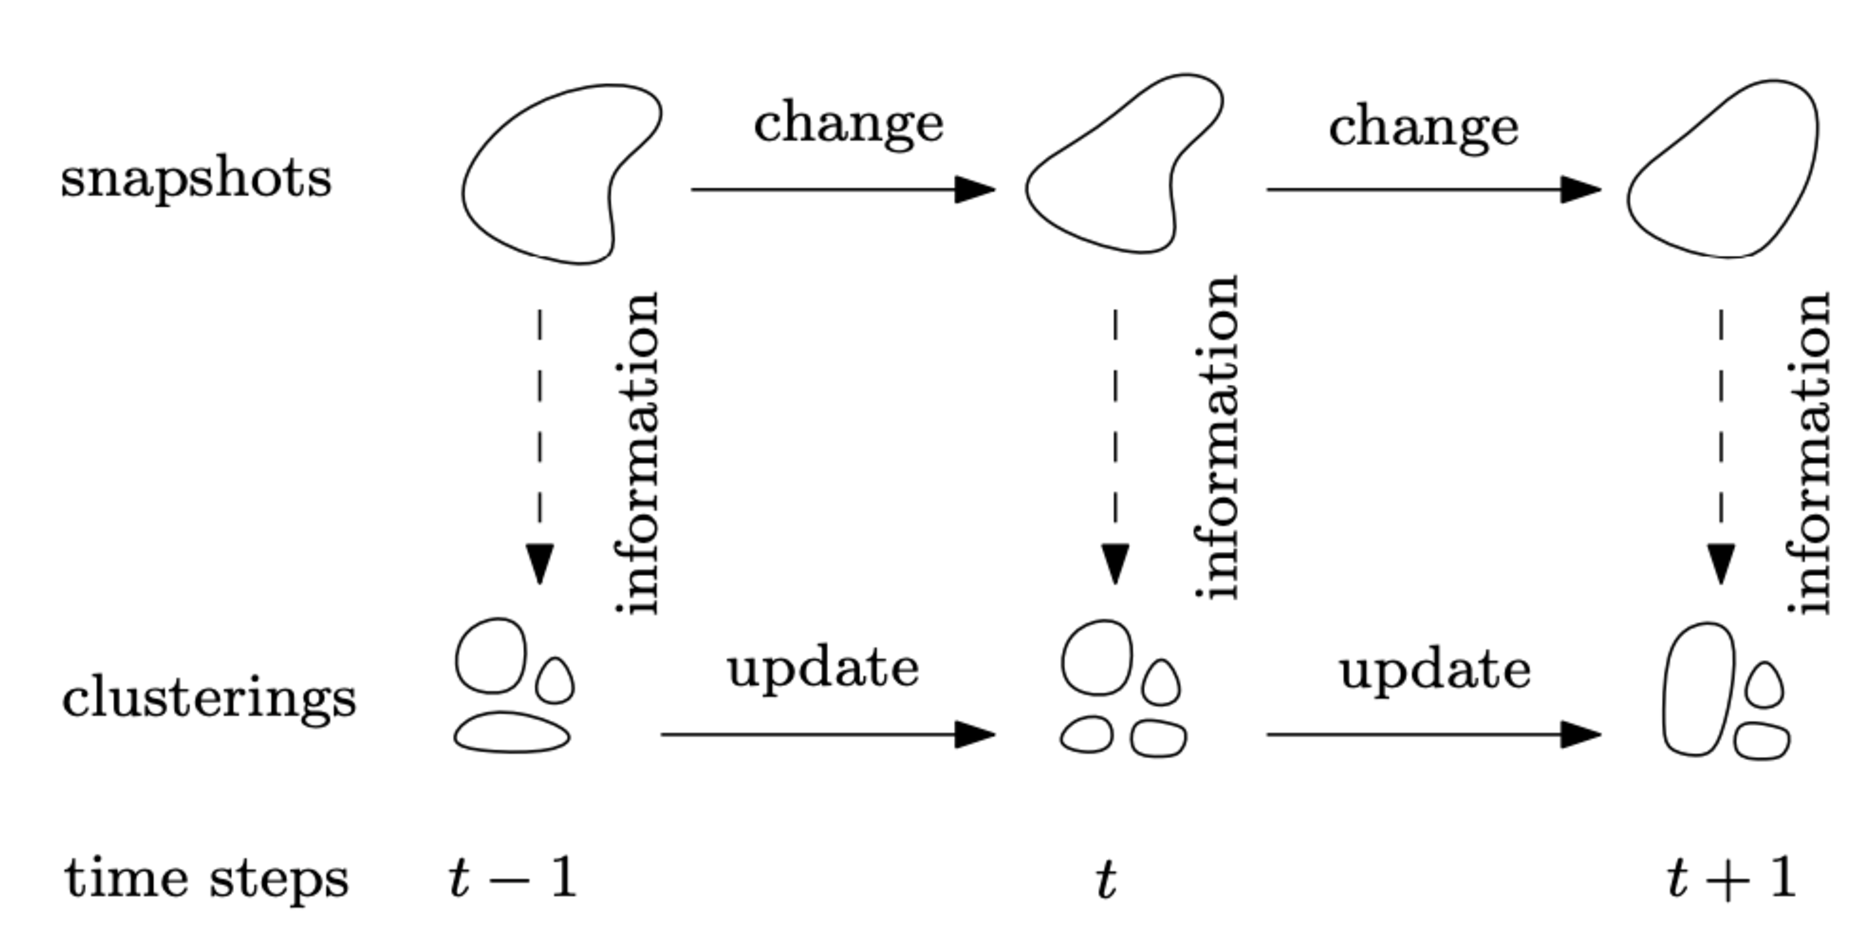
\includegraphics[width=0.9\columnwidth]{img/chapter2/dynamic.pdf} 
 	\caption{Dynamic community detection conventional steps. Figure is contributed from \cite{hartmann2016clustering}.}
 	\label{fig:c2_dynamic}
 \end{figure}  

\cite{chen2013detecting} is a classic study about dynamic community detection. It aims to learn a community matrix $C$ which best depicts the original graph adjacency matrix in a weighted form across all timestamps:
\begin{equation}
	\min_{Y}\sum_t \sum_{i,j}|A_{ij}-\frac{N_i N_j}{2|E|}||Y_{ij}-A_{ij}|
\end{equation}
where $Y=CC^T$.

DYNMOGA model \cite{folino2013evolutionary} is a genetic based approach to detect smooth communities with multi-object optimization. It considers the accuracy of the generated communities in the temporal graph at each timestamp. Meanwhile it also tries to minimize the transformation cost between two community partition results in consecutive timestamps. 

\cite{xu2014dynamic} combines two statistical models: a static model for individual graph snapshot in each timestamp and a temporal model to track the evolution of states. It proposes a prior \& posterior stochastic block model, in which the previously learned parameters in the last snapshot are used to optimize the current community memberships via  extended Kalman filter (EKF). Using similar approaches, SBTM model \cite{xu2015stochastic} leverages hidden Markov assumption in original SBM in which the presence/absence of an edge between two nodes will directly influence whether it will appear again in the next timestamp. 

NEIWalk model \cite{wang2013neiwalk} is a random walk method applied on dynamic content-based graphs by tracking the evolution of both graph structure and node/edge content.  In detail, the model transforms the original graph into a Node-Edge Interaction (NEI) graph which contains two types of nodes and three types of edges. In NEI graph, the two node types are the node and edge in the original content-based graph. And the three edge types are the calculated structural similarity, node content similarity and edge content similarity. The dynamics in the original content-based graph is reflected to the structure evolution in the NEI graph. To detect communities in each timestamp, a random walk based model is proposed to involve a transition probability matrix between each node/edge type and thereafter detect communities in the NMI graph. 

\cite{appel2018temporally} also detects dynamic communities in content-based graphs by incorporating graph structure, content and temporal analysis in a shared matrix factorization model. In each timestamp, it considers to learn three following matrices in a holistic way: a matrix $U_t$ at timestamp $t$ based on both structural and content information, a global  matrix $S$ based on structural information and another global matrix $W$ based on content information across all timestamps. The objective function uses these three matrices to best estimate the original adjacency matrix $A$ and given content matrix $C$:
\begin{equation}
\argmin \sum_{t}||A_t-U_tS^T||^2 + \beta\sum_{t}||C_t-U_tW^T||^2 + \lambda(||S||^2+||W||^2+\sum_t||U_t||^2)
\end{equation}
The first  term aims to estimate $A$, the second term aims to estimate $C_t$ at each timestamp $t$, and the third term is the regularization term  to avoid bias and overfitting.

\cite{wang2013dynamic} focuses on dynamic community detection in graph streams by defining a Local Weighted-Edge-based Pattern (LWEP), which is a subset of node densely connected in local regions. The whole approach is divided into online and offline steps. In the online step, for each node in timestamp $t$, a top-k neighbor node list (with largest edge weights) and a top-k candidate node list (with highest burst activities) are extracted to preserve graph main structure. In the offline step, the LWEPs are created in each timestamp from online results. A straightforward two-step approach first cleans the generated LWEPs and then uses a breadth first search (BFS) method to figure out dynamic community structures.  

\cite{kim2013nonparametric} proposes a nonparametric multi-group membership model for dynamic graphs. Within its model, a community can be tracked as either active or inactive, which is assumed to follows Poisson distribution. In timestamp $t$, the dynamic joining or leaving of a node towards a community is estimated by a Markov chain process considering its previous status in the community. The estimated parameters follow Beta distribution. The community structure can be used to estimate the probability of edge affinities in the original graph. Finally a MCMC method is used to optimize all the to-be-learned parameters under all assumed distributions.

\cite{ghasemian2016detectability} is a theoretical paper which argues a threshold generated from community strength and dynamic change rate. It claims that there would be no effective methods if the dynamic graph has a score below the threshold. Further more, it mathematically proves belief propagation model and spectral clustering are able to detect reliable communities if the graph structure is above the threshold.  

\cite{yang2018poisson} is another statistical work which assumes evolved node-community memberships following Gamma distribution. The communities also follows a Gamma distribution. The edges between nodes follow Bernoulli distribution and their weights follow Poisson distribution. The whole process optimizes all aforementioned distributions through a MCMC process. Similarly,  \cite{peixoto2017modelling} uses Bayesian Markov Chain to generate sequential edges appeared in the graph without specified time windows. 

\cite{delvenne2010stability} introduces a new metric, stability, to assess community partitions. The stability of a community partition is defined as:
\begin{equation}
	r(t,C) = \min_{0 \leq s \leq t} trace[C^T(\Pi M^t -\pi^T \pi)C]
\end{equation}
where $M$ is the node transition matrix, $\pi$ is the normalized degree vector over all nodes and$\Pi = diag(\pi)$ is the corresponding diagonal matrix. $C$ is the community  matrix. The partition with maximized stability may not be the best one in current timestamp. But its community structure should be with good coherence in a relative long time period.

In \cite{gauvin2014detecting}, the time-evolving graphs can be represented as a set of sequential adjacency matrices, which can be integrated as a three-way tensor $\mathcal{T}$. The conventional matrix factorization can be thereafter applied to the tensor by finding three low dimensional matrices $A,B,C$ to best estimate $\mathcal{T}$. $A$ and $B$ provides the graph community structure and $C$ represents the temporal activity of communities. It is a PARAFAC decomposition problem to solve.
\begin{equation} 
\min_{A,B,C} ||\mathcal{T} - A,B,C||^2_F
\end{equation}

\cite{tang2011identifying} focuses on dynamic multi-mode graphs, which is a particular type of heterogeneous graph where the node types and edge connections are constructed from different modes such as text and videos. It uses a matrix factorization approach to learn node community matrix in each timestamp by estimating the interaction between each pairwise modes. And a side effect from snapshot graph in the last timestamp are also considered in the learning process.

\subsection{Large Graph}

Large scale graphs are ubiquitous in various domains. Especially in recent years, with the increasing computation capability, more and more researches focus on how to deal with large graph community detection. A well-known survey paper \cite{harenberg2014community} introduces a number of methods focusing on both overlapping and disjoint community detection as well as many frequently used metrics and datasets for evaluation.

TopGC model\cite{macropol2010scalable} proposes a linear-time searching algorithm to detect the best community instead of the entire graph communities. It uses the idea derived from Locality Sensitive Hashing (LSH) to index nodes and find the communities with largest cluster scores (related to the community size and number of within-community edges). \cite{spielman2013local} is another local searching model which leverages random walks to detect the best community for each given node, and runs in approximately linear time. 

\cite{satuluri2011local} introduces a novel model to deal with large graphs by sparsifying graphs and removing unimportant edges to maintain the main graph structure. Once the graph size is reduced, the running time of most methods will be shortened as their complexity are always related to the graph size. To prune the graph in an efficient manner, a local sparsification algorithm is introduced to maintain the top ranked edges (edge score is calculated by the Jaccard Similarity of current node and the other endpoint node) per node. A further threshold is set up to ensure the pruned graph is still connected. 

\cite{wang2011detecting} formulates a novel problem, community kernel detection, which contains two tasks: find the most influential users and detect their community structure.
It proposes two separate algorithms, GREEDY and WEBA, both to solve the two tasks in a unified framework. In the GREEDY method, it firstly initializes a set of seed nodes as kernel communities. Then these communities expands by merging nodes with closest connections. In the WEBA method, the model learns a weight vector for each node to represent its belonging score to each community. The weight vectors are learned by maximizing the inner product of the vector of all pairwise connected nodes.

GEM model \cite{whang2012scalable} is proposed to cluster large-scale social networks. It consists of three steps: firstly it extracts the main skeleton from the original graph, and then detects the  skeleton graph communities via a k-means method, in the last step the calculated result is propagated back to refine the communities of entire graph. In detail, for graph extraction,  all nodes whose degree are above a threshold are selected and their edges are kept. Then a weighted k-means with refined seeding strategy is applied to cluster the filtered skeleton graph.  In the end, the remained nodes in the original graph are assigned to the generated communities through a breadth first search (BFS) approach.

\cite{li2013efficient} gives a novel definition of a community in which all nodes are closer to the current community centers than to the rest communities. After that, two new algorithms (Cores-Aware and Cores-Unaware algorithm) are proposed to detect communities in linear time. The Cores-Aware algorithm is leveraged under the condition that community cores are known. Then a breadth first search (BFS) approach is applied to calculate other node distances towards all cores and assign their communities. In the Cores-Unaware algorithm, their is no prior-known community cores. 

ESCG model \cite{liu2013large} repeatedly generates supernodes with coarser resolution to replace the original nodes in bipartite graph, which reduces the original graph size and accelerate the running speed. In detail, the model first randomly picks up a number of seed nodes as individual supernodes. Then a BFS approach is taken to allocate the rest nodes to the seed nodes based on their shortest paths. In the end, a standard spectral clustering method is leveraged on the reduced graph to detect communities. 

\cite{de2014mixing} proposes a mixed global and local method to bump up the efficiency via a defined k-path edge centrality as a substitution of the original edge betweeness centrality. Each edge importance score is calculated via random walks, which maps nodes to a latent space and calculates all pairwise distances for final community detection. The k-path edge centrality is defined as:
\begin{equation}
	L^k(e_{ij}) = \sum_{v \ V} Pr(e,v)
\end{equation}
It calculates the sum of probabilities that a k-step random walk passes edge $e_{ij}$ which is originally started as node $v$. And the distance of pairwise nodes can be thereafter calculated as:
\begin{equation}
	d_{ij} = 1 - \sqrt{\sum_{v \in V}\frac{(L^k(e_{vi})-L^k(e_{vj}) )^2}{d(v)}}
\end{equation}
The Louvain method is finally applied on the all pairwise node distances to calculate their communities.

\cite{kollios2013clustering} deals with large probabilistic graphs in which each edge is associated with a probability to appear or not appear. It proposes a simple model to generate a cluster graph $C$ which has the least edit distance with the original graph $G$. And the disjoint subgraphs in the cluster graph $C$ naturally form the communities.

SCD model \cite{prat2014high} is a scalable approach to detect communities by maximizing the Weighted  Community Clustering (WCC) metric. It also allows to run in parallel, which achieves a two-order magnitude acceleration in terms of running speed. WCC is defined based on the intuition that nodes should have a higher chance to form triangles with in-community nodes compared with the out-community nodes. Therefore, for a given node $v$, its WCC score in a community $c$ is calculated as:

\begin{equation}
WCC(v,c) = 
\begin{cases}
\frac{t(v,c)}{t(v,V)} \cdot \frac{vt(v,V)}{|c - v| + vt(x, V-c)} & \text{if t(v,V) $\neq$ 0}\\
0& \text{if t(v,V) = 0}
\end{cases}
\end{equation}
$t(v,c)$ and $t(v,V)$ refer to the number of triangles containing node $v$ in the community $c$ or the whole graph nodes. $vt(v,V)$ refers to the number of nodes that forms close triangles with current node $v$. The sum of all nodes' WCC scores across all communities is the final score to evaluate the fitness of current partition. The paper uses an iterative approach to learn the community partition with largest WCC score. \cite{tsourakakis2017scalable} also takes advantage of closed triangles in a spectral clustering approach.

\cite{li2015uncovering} aims to find overlapping communities in large-scale graphs. It defines a local spectra which uses a set of seed nodes (with known communities) as the dimensions to represent all other nodes through random walks. The local spectra representation hugely reduces the workload to decompose the adjacency matrix. And a refined k-means method helps to group nodes into overlapped communities. 

DFuzzy model \cite{bhatia2018dfuzzy} leverages deep learning techniques in four steps. First, it uses a PageRank method to initialize the potential community centers. Second,  PageRank based clustering encodes node hidden representations by maximizing graph Modularities. Communities are detected in the decoding process by minimizing the reconstruction error in the unified encode-decoder framework.

Some other studies are relevant to large-scale graphs from different perspectives. \cite{hallac2015network} is a theory paper which introduces network lasso to enhance the optimization process. \cite{jeub2015think} is an empirical paper aims to identify under what scenarios that small communities are better/equal/worse than large communities. \cite{peixoto2015model} offers a model selection strategy by considering graph minimum description length. 

\subsection{Attribute Graph}

\begin{figure}
	% \setlength{\belowcaptionskip}{-10pt}
	\center
	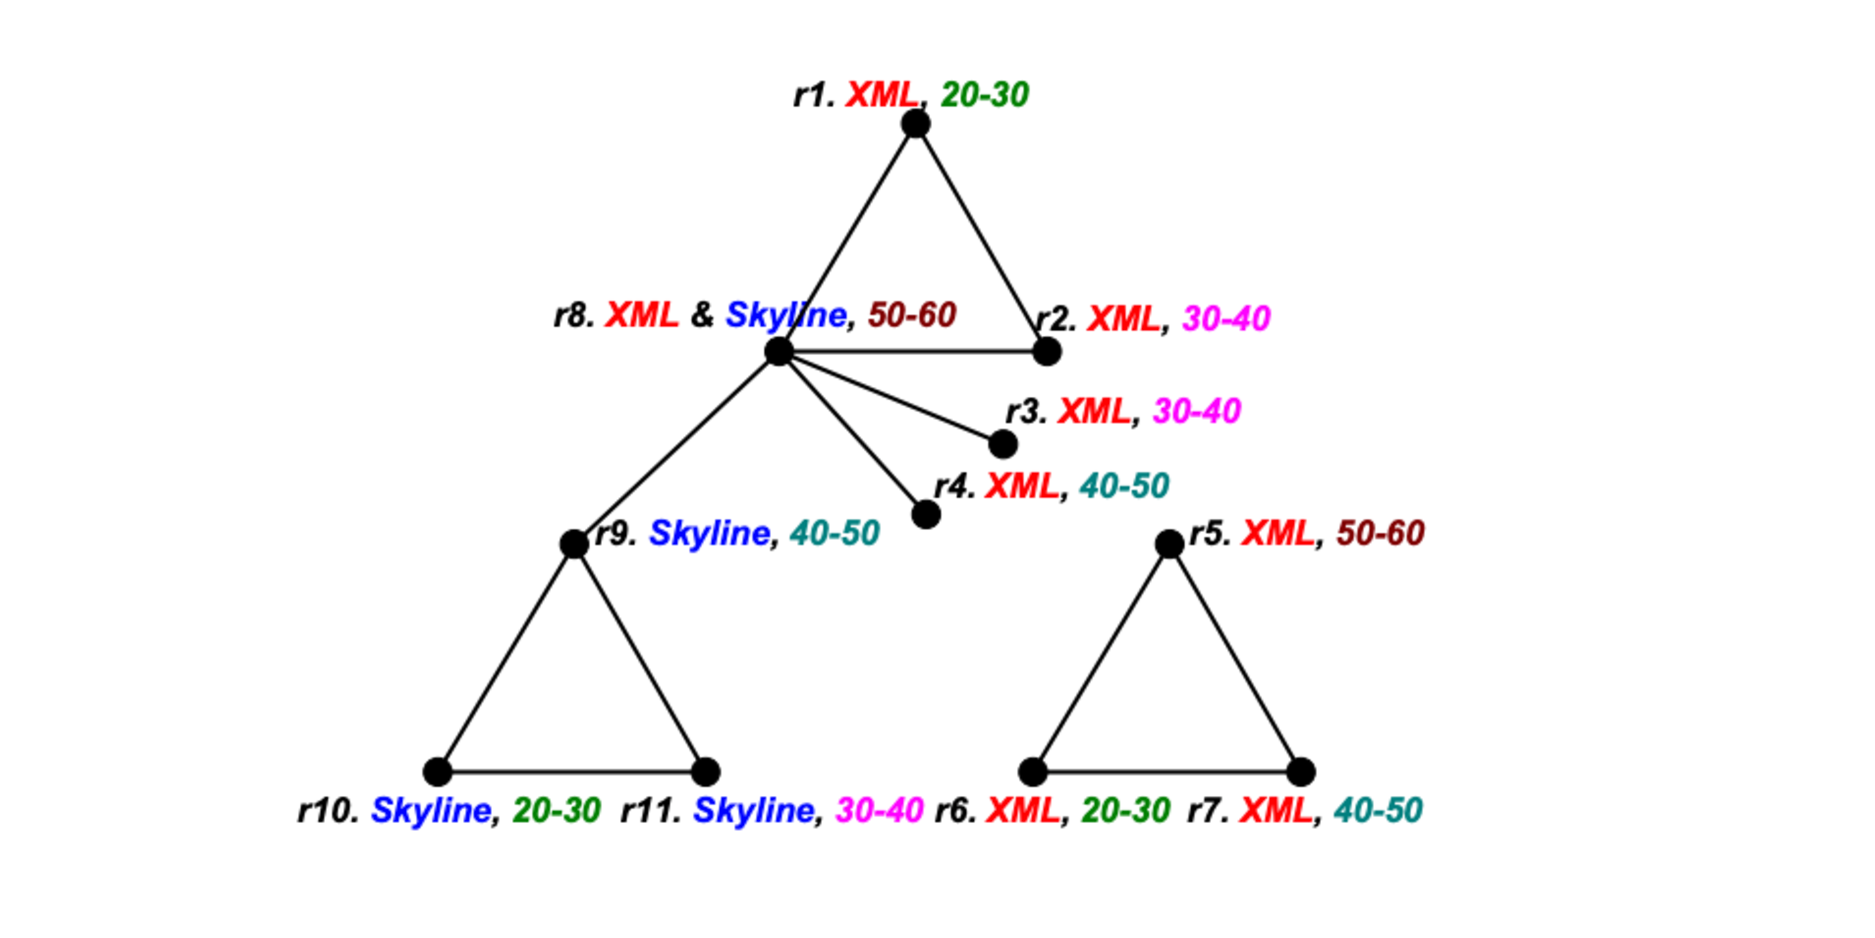
\includegraphics[width=\columnwidth]{img/chapter2/attribute.pdf} 
	\caption{A co-author graph with two attributes ``Topic'' and ``Age''. Figure is contributed from \cite{yang2013community}.}
	\label{fig:c2_attribute}
\end{figure}  


Intuitively, attribute graph is a type of graph in which nodes contains extra information. Figure \ref{fig:c2_attribute} shows a typical attribute co-author graph with ``Topic'' and ``Age'' attributes. An attribute graph $G(V,E)$ is associated with an attribute collection $\Lambda=\{ \lambda_1,...,\lambda_m\}$ containing $m$ different attributes.  Each node $v$ is associated with an attribute vector $[\lambda_1(v),...,\lambda_m(v)]$ where $\lambda_1(v)$ is the attribute value of node $v$ on attribute $\lambda_m$. A more complex attribute graph can involve attributes in edges as well with similar representations to node attributes.  Bayesian approaches and nonnegative matrix factorization approaches are the two main tracks of methods, and their related works are summarized in Table \ref{tab:c2_attribute}.

\begin{table}
	% \scriptsize
	\centering
	%   \vspace{-3em} 
	% \renewcommand{\tabcolsep}{2pt}
	\begin{tabular}{|p{5cm}|p{9cm}|} \hline
		\textbf{References} &  \textbf{Main Idea} \\ \hline
		\cite{xu2012model,han2015probabilistic,bojchevski2018bayesian,he2017joint} & Bayesian generative \& probabilistic model\\ \hline
		\cite{qi2012community,wang2016semantic,qin2018adaptive,}& Nonnegative matrix factorization\\ \hline
		\cite{zhang2019attributed,jin2019graph}& Graph convolutional network \\ \hline 
		\cite{zhou2010clustering,pool2014description,yang2013community,huang2015dense}& Others\\ \hline 
	\end{tabular}
	\caption{The main ideas of mainly introduced attribute graph community detection approaches.}
	\label{tab:c2_attribute}
	
\end{table} 


Inc-Cluster model \cite{zhou2010clustering}  uses random walk distance matrix instead of adjacency matrix to calculate node communities. The random walk distance matrix considers the random walk probability between each pair of nodes and their involved attributes. Thereafter, a Kmeans-like method is taken to initialize community centroids and run with the four following steps iteratively until convergence: first,  it assigns nodes to the community with the nearest centroid random walk distance; second, it updates each community centroid from the newly formed communities; third, it adjusts attribute weights with an efficient incremental method; fourth, it re-computes the random walk distance matrix and starts the next iteration. 

SCMAG model \cite{huang2015dense} aims to retrieve the dense communities from attribute graphs. It firstly leverages an entropy-based method to find dense subspaces. A random walk based method calculates the structural closeness and attribute similarity between communities together as a unified metric. A combining strategy is finally proposed based on the metric to merge subspaces together as communities. 

\cite{xu2012model} seamlessly captures both structural and attribute aspect information and develops a Bayesian probabilistic model to detect node communities. It leverages three matrices including adjacency matrix $X \sim Bernoulli(\cdot)$, attribute matrix $Y \sim Multinomial(\cdot)$ and node community label vector $Z \sim Multinomial(\cdot)$. The overall generative process firstly samples the community label for each node. Then given the community label and node itself, the model samples node attributes. In the end, given community labels for each pair of nodes, the model samples whether there is an edge between them. The overall idea is to reproduce the original graph by optimizing these three generation probabilities.

CRM model  \cite{han2015probabilistic} is also a probabilistic model to incorporate all user information from social networks. The overall approach aims to generate three types of user information including community (each edge belongs to a community), role (each node can have multiple roles) and action (edge node can take multiple actions such as transferring a message). The three generative process are interacted with each other and optimized through an EM approach. 

PAICAN  \cite{bojchevski2018bayesian} is a jointly model which learns partial node anomalies and communities via a statistical inference perspective. A node is a partial node anomaly when it is an outlier in at least one attribute. In the graph generative process, an edge is generated from different distribution assumption under three case of endpoint node information: both nodes are good,  one endpoint node is good, and both nodes are anomaly. \cite{he2017joint}  is another model involving node semantics. Similarly, the overall process is a joint community $\rightarrow$ edge generation and topic $\rightarrow$ attribute generation model.
 
\cite{pool2014description} aims to detect top $k$ communities which can both group cohesively connected nodes together and concisely describe their attributes. It defines two types of errors to assess community partition fitness. The first type error is missing edges between nodes in the same community. The second type error is the edges existing between communities. The model calculate the scores of community given these two criteria. The idea of this paper is to generate concise queries from node attributes and selects top $k$ best fit communities for these queries. 

CESNA model \cite{yang2013community} detects overlapping communities by considering both edge structure and node attributes. It is a scalable algorithm with linear running time. The intuition behind CESNA model is that node community memberships should be able to indicate node attributes. The probability that a node $u$ contains attribute $k$ is described as:
\begin{equation}
	P_{uk} = \frac{1}{1+exp(\sum_c W_{kc}\cdot F_{uc})}
\end{equation}
where $F_{uc}$ is the affiliation score that node $u$ belongs to community $c$. Weight $W_{kc}$ is the weight factor for attribute $k$ towards community $c$.

\cite{qi2012community} shows how edge content can be used to improve the effectiveness of community detection. The overall model is derived from matrix factorization. It considers to minimize both structural object and edge content object in a unified function $\mathcal{O}(E)$:

\begin{equation}
\mathcal{O}(E) = ||E^TE\Delta - \Gamma||^2_F - \lambda tr(E^TLE)
\end{equation}

The first part is the structural object to minimize, where $\Gamma$ is a $|E|\cdot|V|$  matrix to encode edge and node underlying structure. $\Gamma_{ij} = 1$ if $v_j$ is the start-or end-point of $e_i$. Otherwise $\Gamma_{ij} = 0$. $E$ is a low dimensional matrix representation for all edges. $\Delta$ is a  $|E|\cdot|V|$  matrix whose entry $\Delta_{ij} = \frac{1}{d(vj)}$ if $v_j$ is the start-or end-point of $e_i$. The second part is the edge content object. $tr(\cdot)$ denotes the trace of relevant matrix. $\lambda$ is a weighting factor. $L$ is the normalized Laplacian matrix storing all pairwise edge content similarities. In the end, edge vectors are learned  and used for community detection.

\cite{wang2016semantic} aims to learn a community membership matrix $U$ and community attribute matrix $C$ through a nonnegative matrix factorization framework. The objective function in this model is defined as:
\begin{equation}
	\argmin_{C \geq 0, U \geq 0}||U-SC||^2_F + \alpha\sum_{j=1}^{k}||C(:,j)||^2_F + \beta ||A-UU^T||^2_F
\end{equation}
where $U_{ij}$ is the propensity of node $i$ belongs to community $j$. $C_{qr}$ is the propensity of that attribute $q$ belongs to community $r$. $S$ is the given node attribute matrix. The first term aims to estimate node community membership matrix from node attributes. The second term is an add-on bias. The third term is to use community membership matrix to estimate the original adjacency matrix $A$.

\cite{qin2018adaptive} incorporates node content into a nonnegative matrix factorization approachc and use a weight matrix $C$ to control the impact of the attribute information for community detection. The objective function it aims to optimize is as:
\begin{equation}
\argmin_{X \geq 0,Y \geq 0} \alpha ||A-XX^T||^2_F + ||X-CY||^2_F
\end{equation}
where $A$ is the adjacency matrix, $X$ is the community membership matrix, $Y$ is the community attribute matrix to describe how much likely the community can be described by each attribute. $C$ is the node attribute matrix. Both $X$ and $Y$ are the matrices to be learned. 

\cite{zhang2019attributed,jin2019graph} are both deep-learning based method to involve node attribute into graph convolution process and trained in an end-to-end manner.

\subsection{Summary}
In this section, I introduce five different types of graphs and a bunch of related research works. Some of the graph types are commonly seen in real-world scenarios such as sparse and large graphs. Effective and efficient models on such graphs can produce huge practical value to reduce online latency and required machine memories. Researches in attribute graph is becoming more popular because it can involve extra information to support graph partition. The extra information is always with meaningful semantics, clear format and easy to be obtained.  Besides the type of graphs introduced in this section, there are also other types of works, such as signed graph and hypergraph, which are all interesting topics and deserves more future exploration.  
\section{Tasks}
In this section, research works about five  popular community detection tasks are summarized. The five selected tasks are independent with each other and tackle community detection problems from various perspectives. 

\subsection{Overlapping Community Detection}
\begin{figure}
	% \setlength{\belowcaptionskip}{-10pt}
	\center
	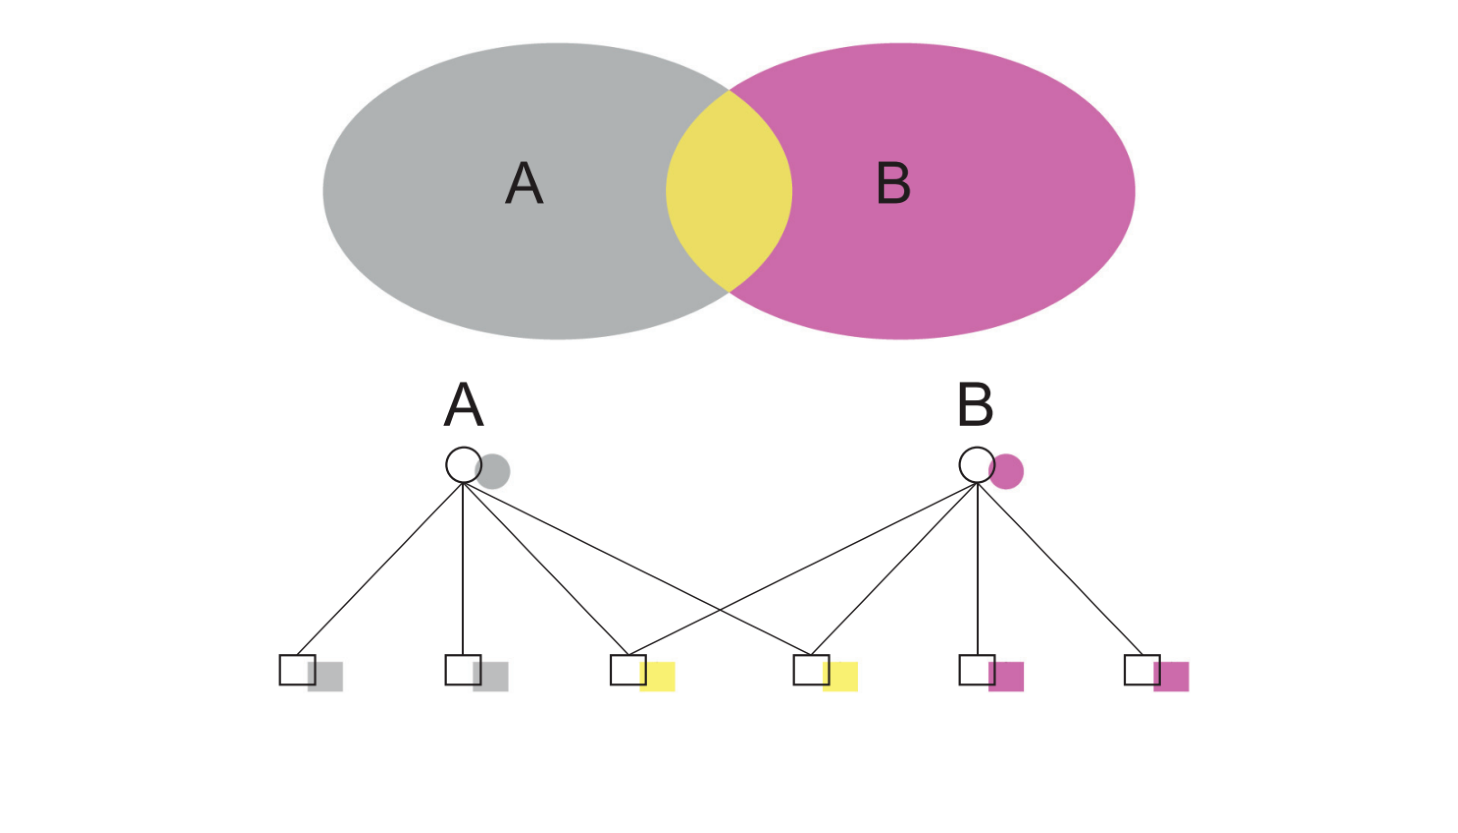
\includegraphics[width=\columnwidth]{img/chapter2/overlapping.pdf} 
	\caption{Overlapping Community Structure where nodes can belong to multiple communities. The figure is contributed from \cite{yang2013overlapping}.}
	\label{fig:c2_overlapping}
\end{figure}  


Overlapping community detection is one of the most fundamental topics and many relevant studies are published. By definition, a node $v$ can belong to multiple communities simultaneously so as to cause the overlaps between communities. Figure \ref{fig:c2_overlapping} visualizes the community structure under overlapping circumstance. The nodes marked in color yellow are affiliated with both community $A$ and $B$. Table \ref{tab:c2_overlapping} categorizes and summarizes the focus of each mentioned study for overlapping community detection.

\begin{table}
	% \scriptsize
	\centering
	%   \vspace{-3em} 
	% \renewcommand{\tabcolsep}{2pt}
	\begin{tabular}{|p{5cm}|p{9cm}|} \hline
		\textbf{References} &  \textbf{Main Idea} \\ \hline
		\cite{coscia2012demon,whang2013overlapping,whang2016overlapping,huang2018overlapping,wang2017overlapping} & Local search and seed expansion\\ \hline
		\cite{yang2013overlapping,zhang2015incorporating,zhang2016modeling,eustace2015overlapping,jin2015combined}& Nonnegative matrix factorization\\ \hline
		\cite{gopalan2013efficient,jin2016detect,}& Bayesian, generative model\\ \hline
		\cite{yang2012community}& Affiliation network\\ \hline
	\end{tabular}
	\caption{The main ideas of mainly introduced overlapping community detection approaches.}
	\label{tab:c2_overlapping}
	
\end{table} 

\cite{amelio2014overlapping} is a survey paper published in 2014. Although the methods introduced within it are sort of dated, it still offers covers several main track methodologies (node seed and local expansion, clique expansion, and label propagation) and particular scenarios (link clustering and dynamic graphs). It draws a conclusion that there is no universal method to deal with all types of graphs with different characteristics in sparsity, degree distribution, and overlap percentage among communities. In the end, it also points out two essential questions to be solved for later researchers, which is ``when to apply overlapping methods and how significant the overlapping is''.  \cite{xie2013overlapping} is another authentic survey paper which reviews a set of methods, benchmarks and evaluation metrics. Besides that, it also reviews papers using stochastic block model or density based models. To study the performance differences among models,  it introduces several benchmark graphs in which node ground truth community is known, i.e. LFR benchmark graph\footnote{https://sites.google.com/site/andrealancichinetti/files}. A set of evaluation metrics including Normalized Mutual Information (NMI) and Omega index are introduced as well. Meanwhile, empirical studies are applied and evaluated on all aforementioned methods using different benchmark graphs. In the end, the paper discovers the sensitivities of different models in sparse graphs appeared in real-world social networks.

DEMON model \cite{coscia2012demon} unveils its overlapping communities with a local-first approach by grouping ego neighbor nodes into the same clusters and finally merges the local communities into a global collection. In the local-first grouping process, DEMON applies a EgoMinusEgo function to first extract ego-based subgraphs for each node $v$ where the node set is node $v$ and all its neighbor nodes $\mathcal{N}(v)$  and the edge set is all graph edges between the selected nodes ($v$ and $\mathcal{N}(v)$). After that, each ego-based subgraph will remove the node $v$ and all its associated edges to achieve an EgoMinusEgo subgraph. An label propagation community detection method is subsequently applied on each EgoMinusEgo subgraph and select a set of largest clusters to best cover the entire graph. In the end, a merging process is applied on the previously generated clusters according to their node similarities and construct the final community partition result. LOSP model \cite{he2015detecting} is another method to explore local neighborhood structures of each node. It defines a Local Spectral Subspace using the first $d$ eigenvectors from the normalized adjacency matrix. In each potential community $c$, a set of seed nodes are given, and an iterative process is applied with the help of seed nodes and the Local Spectral Subspace to rank the top $N_c$ nodes with highest random walk probabilities to appear in the current community. Those nodes are finally regarded as other latent members in each community $c$. 

LOSP model offers a great insight to use seed node expansion to detect overlapped communities. Inspired by LOSP model, \cite{whang2013overlapping,whang2016overlapping} propose a four-phase model including filtering, seeding, seed set expansion, and propagation. The natural of the model first filters out the regions of the graph which don't involve overlapping structure. A seeding strategy inspired by Kmeans selects a set of seed nodes with small Conductance relationship. A seed set expansion approach is further applied by taking advantage of personalized PageRank model to construct raw communities near each seed node. In the last propagation step, the raw communities are expanded again to the regions previously removed in the filtering phase. Similarly, \cite{yang2017finding} also designs a new seeding strategy and expands a set of nodes from seed nodes via a personalized PageRank model. Thereafter it develops a model on the expanded nodes to detect overlapped communities. The seed nodes are the nodes in the maximum spanning tree of the original graph. Personalized PageRank model helps to expand the seed nodes and merge them into raw community structure by maximizing modularity score of the graph. The last optimization step is to merge communities when the shared node ratio of two communities is above an overlapping threshold.

OCD-HSN model \cite{huang2018overlapping} contains a seed selection step as well as community initialization and expansion step to group nodes into clusters in an efficient manner. It claims to be the first research work for overlapping community detection in heterogeneous graph containing both undirected and directed edges. Based on user semantic interests and social connections, this study constructs a heterogeneous graph to hold all types of user profiles. A set of seed nodes are selected based on their centrality and conductance in the graph. The neighbor nodes of the seed nodes naturally  construct overlapped communities. Later on, a fitness evaluation process is leveraged to add or remove nodes  based on the node connectivity in each community. 

Structural centers are defined and utilized in \cite{wang2017overlapping} to support local expansion for overlapping community detection, which are the nodes that have high node degrees and are also far away from other structural centers.


By natural, nonnegative matrix factorization can solve overlapping community detection problem as it can directly learn low dimensional node representation matrix from the graph matrices such as adjacency matrix. Each column in the reduced node represention matrix represents an eigenvector, which also can be regarded as a community. Therefore, the learned node representation can be regarded as the node affiliation distribution over communities. BIGCLAM model \cite{yang2013overlapping} is a classic overlapping community detection model which can take care of large-scale graphs. In its model, $F$ represents a nonnegative matrix where $F_{uc}$ is the affiliation score of node $u \in V$ in community $c \in C$. Given an unlabeled and undirected network $G(V, E)$, BIGCLAM aims to re-generate all graph edges using node's community affiliation distribution. It aims to maximize the probability of node $u$ and $v$ if there is an edge between them and minimize the probability if there is no edge.  Therefore, the objective function $l(F)$ to maximize turns to be:

\begin{equation}
l(F) = \sum_{(u,v) \in E} log(1-exp(-F_uF_v^T)) - \sum_{(u,v) \notin E} F_uF_v^T
\end{equation}

The number of communities can also be determined in the model through an empirical test.
 
PNMF model \cite{zhang2015incorporating} is also a nonnegative matrix factorization model.  Unlike conventional matrix factorization models to directly decompose the original adjacency matrix, PNMF considers the situation that a node prefers its neighbor nodes. Therefore, instead of re-generating the edges between two nodes, this paper considers node triplet $(i,j,k)$.  $j>_{i} k$ denotes that $ j \in \mathcal{N}(i)$ and $k \notin \mathcal{N}(i)$ so that node $i$ prefers $j$ to $k$. And the overall goal of this approach is to maximize this preference likelihood that neighbor nodes should be preferred than non-neighbor nodes:
\begin{equation}
\begin{aligned}
l(F) &= \sum_{(i,j,k) \in S} log(p(j>_{i}k|F) )-\lambda \cdot reg(F) \\
 &=  \sum_{(i,j,k) \in S} log(\sigma(F_iF_j^{T} - F_iF_k^{T}))-\lambda \cdot reg(F)
\end{aligned}
\end{equation}
 where $S$ is pre-sampled node triplet collection which satisfies the node preferences. $reg(F)$ is the regularization term added to avoid overfitting and $\lambda$ is the regularization weight.
 
HNMF \cite{zhang2016modeling} is another nonnegative matrix factorization model which considers both-sided relationships between edges and communities. From the community-to-edge perspective, it takes advantages of PNMF model to maximize the log likelihood of node connection preferences in all sampled node triplets. From the edge-to-community perspective, it uses negative sampling strategy in a skip-gram model to maximize the probability if two nodes are neighbor nodes and minimize the probability if they are not. The final loss is the loss sum from both PNMF and the negative sampling, which is aimed to be maximized in the joint training process. 
 
NRATIO model \cite{eustace2015overlapping} generates a vertex neighborhood ratio matrix to substitute original adjacency matrix or Laplacian matrix. This matrix refines the graph adjacency matrix where two nodes are connected only if their common neighbor nodes surpasses the average number of neighbors in all pairwise nodes. In the next step, nonnegative matrix factorization is applied on the refined matrix to learn a community distribution over each node. As the vertex neighborhood ratio matrix reduces the influence of unrelated nodes in community structures, the number of data points in the matrix are significantly reduced, which fastens the running speed.

\cite{jin2015combined} first describes a stochastic block model to accommodate both node and edge communities, and then uses conductance measurement to fine-tune the learned node community distribution. One outstanding point of this paper is that the model considers edge communities. By definition, in the adjacency matrix $A$, $a_{ij} = 1$ if node $v_i$ and node $v_j$ are connected through an edge. And, in bipartite graph matrix $B$, $b_{ij} = 1$ if node $v_i$ and edge $e_j$ are directly linked each other. The paper aims to learn a node community affiliation matrix $H$ where $h_{ij}$ denotes the propensity of node $v_i$ belonging to community $c_j$ and an edge community affiliation matrix $W$ where $w_{ij}$ denotes the propensity of edge $e_i$ belonging to community $c_j$. In the end, to use the node/edge community information ($W$ and $H$) to re-construct the two matrices $A$ and $B$, the objective function is defined as follows:

\begin{equation} 
	\mathcal{O}(H,W) = ||A-HH^T||^2_F + \lambda ||B-WH^T||^2_F
\end{equation}
where $||\cdot||_F$ is the Frobenius norm, $H$ and $W$ have to be nonnegative matrices.

AGM model \cite{yang2012community} is a preliminary study using affiliation network to re-generate the original social network. Given only the overlapping community affiliation of each node, it learns the  reproduction of original links between nodes in order to construct the social network. The edge generation probability is defined as: 
\begin{equation}
p(u,v) = 1-\prod_{c \in C_{uv}} (1-p_c)
\end{equation}
where $C_{uv}$ are a set of shared communities for node $v$ and $u$. $p_k$ refers to the probability of an edge forming between two nodes in the community $c$. 

\cite{gopalan2013efficient} uses a mixture membership stochastic block model to learn node overlapping communities. The overall framework is a Bayesian approach. It assumes the overlapped community memberships of each node $v_i$ is associated with a Dirichlet distribution $\theta_i$. For each pair of node $v_i$ and $v_j$, it draws a community indicator $z_{i \rightarrow j}$ from node $v_i$’s community membership $\theta_i$ and then draws  a community indicator  $z_{i \leftarrow j}$  from node $v_i$’s community membership $\theta_j$. Each indicator points to one
of the $|C|$ communities. Finally, it draws an edge between two nodes with the generation probability:
\begin{equation} 
p(y_{ij} = 1|z_{i \rightarrow j},z_{i \leftarrow j}) =
\begin{cases}
z_{i \rightarrow j},       & \quad  z_{i \rightarrow j} = z_{i \leftarrow j}\\ 
\epsilon,  & z_{i \rightarrow j} \neq z_{i \leftarrow j}\\ 
\end{cases}
\end{equation}
The whole process is optimized and all nodes' $\theta$ are learned by maximizing the edge generation probability $p(y_{ij} = 1)$from the actual graphs.  $\epsilon$ is a small constant. The
parameter $\beta_{z_{i \rightarrow j}}$ is the density of community $z_{i \rightarrow j}$.

Similarly, \cite{jin2016detect} also introduces a Bayesian based generative model. It assumes a Poisson distribution for node community distribution and is optimized using a Expectation-Maximization (EM) approach. Node communities are selected according to its learned community distribution and related community conductance in the end.

\subsection{Number of Communities}
Among all sorts of community detection models, only few of them can automatically determine the number of communities given the model nature. Most of them need to specify the community number in advance before applying their main processes. Therefore it is still an open question about how to choose the exact community number. Many in-depth researches draw their conclusions either from empirical studies or mathematical proofs. In this section, several works particularly exploring this research question are introduced and discussed, which offers general insights for potential community number selection.

\cite{newman2016estimating} proposes a statistical model using Bayesian inference analysis. It finds the correct number of communities by maximizing the integrated likelihood of graph structure and observed community partition using a generative model. In detail, given the prior knowledge of graph structure (adjacency matrix $A$) and community partition $C$, it uses Markov chain Monte Carlo (MCMC) importance sampling to calculate the posterior distribution of community number $|C|$.

\cite{le2015estimating} develops an efficient model to study community numbers based on graph spectral properties. It statistically proves the number of positive and most informative eigenvalues as the estimated number of communities on five spectral clustering methods which use either the non-backtracking matrix or the Bethe Hessian matrix. 

Moreover, two motivations happened in stochastic block models urge the exploration of community numbers. First, edges are not necessarily independent if only the communities of their endpoint nodes are given. Second, the loss of precision occurred in spectral clustering is inevitable. Therefore, through a set of rigorous proofs, \cite{saldana2017many} proposes a composite likelihood BIC (CL-BIC) model to handle the community number selection  happened in stochastic block model (SBM), degree-corrected block model (DCBM) and mixture-membership block model (MMB). 

For other works relevant to community number selection, \cite{kawamoto2017cross,chen2018network} both leverage the leave-one-out cross-validation to determine the community number by optimizing the edge prediction error and Bethe free energy in stochastic block model.  \cite{kawamoto2018comparative} conducts a comparative analysis on various community detection models (stochastic block model, greedy methods, statistical inference models and spectral methods) to track the changes of assessment criteria (modularity, map equation, Bethe free energy and prediction error and isolated eigenvalues) associated with various of community numbers.

\subsection{Community Search}
Instead of generating communities for all nodes in the graph, community search based approaches aim to find the top relevant subgraphs or communities that match particular purposes, which can be regarded as a mixture of community detection and information retrieval. Currently, there are two main types of search scenarios. One is that given a set of query nodes, return the densest subgraph containing query nodes. The other is given a set of query nodes, return their top $k$ most relevant communities. Relevant works are summarized by main ideas in Table \ref{tab:c2_search}.

\begin{table}
	% \scriptsize
	\centering
	%   \vspace{-3em} 
	% \renewcommand{\tabcolsep}{2pt}
	\begin{tabular}{|p{4.5cm}|p{9.5cm}|} \hline
		\textbf{References} &  \textbf{Main Idea} \\ \hline
		\cite{sozio2010community,cui2014local,barbieri2015efficient,wu2015robust,huang2015approximate} & Return the densest subgraph containing all query nodes\\ \hline
		\cite{chen2012dense,qin2015locally,lancichinetti2011finding,huang2014querying,zheng2017finding,yan2019constrained,li2015influential}& Return top $k$ most relevant/influential communities with or without query nodes \\ \hline 
	\end{tabular}
	\caption{The main ideas of community search approaches.}
	\label{tab:c2_search}
	
\end{table} 


\cite{sozio2010community} is a very classic paper of community search, which is defined as given a graph $G(V,E)$ and a set of query nodes, seeking a a subgraph of $G$ which contains all the query nodes and meanwhile is densely connected. The nodes with trivial degrees and far away from query nodes are filtered out from the community. The final goal of this paper is to maximize the minimum degree of a subgraph containing all query nodes. A greedy solution is proposed by deleting each node with minimum degree at each step. The iterative process terminates either at least one of the query node reaches to the minimum degree or is no longer connected with the rest of nodes. Further two heuristic approaches are extended to detect the community with an upper bound size restriction. 

\cite{cui2014local} is a subsequent work of the previous one, which aims to detect the best community for a given node. It formulates and solves two community search problems: communitysearch with a threshold constraint (CST) problem and community search with a maximality constraint (CSM) problem. Two approaches including global search and local search are proposed where the second approach is more efficient than the first one because of reducing searching space significantly.  

\cite{barbieri2015efficient} is another follow-up work of \cite{sozio2010community}. It improves the model efficiency and accuracy as one limitation of the previous work  is that it tends to find quite large solutions, which negatively affects the detected community accuracy. Unlike the \cite{sozio2010community} in which the community size is constrained, it aims to detect the smallest-size community among all optimal ones. In detail, it computes the core decomposition and organizes the retrieved k-cores (maximal subgraphs where each nodes are connected at least $k$ other nodes in a subgraph). In the end, a greedy-connection approach is leveraged to use a local search method to reduce the potential subgraph size (greedy step) and a Steiner Tree-based strategy to find the minimum number of nodes that make all query nodes connected.
 
Given a query node, \cite{wu2015robust} formulates a query biased densest connected subgraph (QDC) problem which aims to find the densest subgraphs that contains the query nodes and is also internally connected. A densest subgraph can be regarded as a local community in this paper. To reduce a free rider effect which involves irrelevant nodes into densest subgraphs, a random walk based weighting scheme is proposed to set higher penalties to these irrelevant nodes when they are included in the subgraphs/communities. 

\cite{huang2015approximate} solves a closest truss community (CTC) problem which finds a connected k-truss subgraph with the largest $k$ and minimum graph diameter.  By its definition, a k-truss subgraph requires each edge is contained in at least $k-2$ triangles  in the subgraph. A greedy algorithm is proposed to first find a raw CTC that contains all query nodes, then iteratively removes the furthest nodes in the CTC to finally achieve the optimized subgraph.
 
\cite{chen2012dense} introduces a partial clustering model to extract the most dense subgraphs, meanwhile it does not require to determine the number of subgraphs in advance. The model is inspired by the matrix blocking problem to reorder the adjacency matrix $A$ and to find the dense diagonal blocks as extracted subgraphs. It considers three types of graph scenarios including undirected graph, directed graph and bipartite graph. By calculating the pairwise columns in the adjacency matrix, it obtains the similarities between all pairs of nodes, which is stored as matrix $M$. The final goal turns to reorder the rows and columns of $M$ so that inside each nontrivial diagonal block of matrix $M$, there exists at least one datapoint larger than a threshold for each row and column. It means that for each node in the diagonal block, there exists at least one other node densely connected with it. To accelerate the running speed, a hierarchical optimization approach is proposed in a top-down manner. The large generated diagonal blocks are finally regarded as extracted dense graphs. 

 \cite{qin2015locally} aims to retrieve top $k$ locally densest subgraphs (LDS) which are particularly defined in the paper. LDS is defined based on density (nodes within the LDS are densely connected) and compactness (removing a node in LDS will lose significant number of edges within it). With solid proofs, LDS  should satisfy a set of structural properties in compactness, cohesive and disjoint property. The original optimization approach is based on greedy algorithm, which runs in polynomial time. To reduce this running time, three optimization strategies are applied including pruning invalid nodes, optimization in finding dense subgraphs and optimization in verifying whether the dense graphs are eligible LDS.
 
OSLOM model \cite{lancichinetti2011finding} finds statistically significant communities through local optimization of a fitness function (significance score) which considers single cluster analysis and full network analysis. In single cluster analysis, the significance of a community is defined as the probability of finding the community in a random null model. In full network analysis, an iterative approach is leveraged to optimize the whole graph-level significance score by grouping nodes into proper communities. The approach first adds external nodes to existing subgraphs based on the generative probability. After that non-significant nodes are removed from the updated subgraphs.  

\cite{huang2014querying} regards a node as a query in the graph, and retrieves its k-truss communities through a designed compact and elegant index structure, which makes the overall model scalable with linear cost to serve online community search tasks.  On top of k-truss subgraph, k-truss community is defined with an extra edge connectivity constraint to ensure its node connectivity, which is any two edges in a k-truss community should either belong to the same triangle, or are reachable from each other through a series of adjacent triangles. To accelerate the running speed, a simple k-truss index are developed using an existing truss composition algorithm. Further an enhanced TCP-index is proposed to avoid two drawbacks from previous index: unnecessary access of dis-qualified edges and repeated access of qualified edges. 

Having the same research goal, \cite{zheng2017finding} takes edge weights into account to support better k-truss community detection for query nodes. It firstly utilizes a Breadth first search (BFS) method by removing unimportant edges iteratively. However this BFS approach suffers high computational cost which can not deal with large scale graph. To tackle this problem, it designs a KEP-index (Key Edges Preserved Index) which stores all possible k-truss community candidates in a space-efficient index structure. In the index construction process, communities are decomposed (edges are removed) in a hierarchical manner and the related key edges to reconstruct the hierarchical community tree are stored in the tree-shaped index. 

\cite{yan2019constrained} takes advantages of random walks to detect local graph communities. Starting from a set of seed nodes with given community memberships, the method labels each seed nodes with same/different colors according to its community. And a color-based random walk is applied to propagate colors across nodes to detect all other nodes communities. To store the color of each node, $K$ transition matrices are maintained where $K$ refers to the number of distinct colors in the seed nodes. Throughout an iterative propagation process, the color of each node can be learned and updated by its last-iteration color and the propagated colors from its neighbor nodes. The final color of the nodes are their deterministic community labels. 

Derived from k-core, \cite{li2015influential} proposes an online search algorithm to find the top k-influential communities in linear time through a linear-space index structure. A k-influential community means each node weight within should be at least $k$. The paper introduces a basic algorithm, a depth first search (DFS) and a final index based algorithm. The index based algorithm is able to handle large networks and runs in linear time. It uses a tree/forest index structure to hold all k-influential communities and utilizes a DFS function to iteratively add/remove nodes for index organization until all possible communities are scanned. 

\subsection{Community Detection Enhancement}

Enhancing community detection performance is also an essential task as it provides extra in-depths supports to explore how to improve model performance. As there is no main trend in this research topic, different types of approaches are introduced here with dispersive solutions, including assigning edge weights, removing unimportant nodes, or involving external information, etc. 

\cite{khadivi2011network} assigns proper edges weights on unweighted graphs to circumvent resolution limit \& extreme degeneracy problems and in the end enhances the performance of modularity based methods. modularity has been proved to suffer a resolution limit problem that the community size is constrained. With solid proofs, applying a weighted modularity can increase the upper bound and decrease the lower bound of community size. It allows to detect both larger and smaller communities using weighted modularity methods. Extreme degeneracy problem means that it goes more and more difficult to find the optimal community partition when the community size is large. And a proper weighting schema is able to strength the intra-community edges and weaken the rest to better clarify the community boundary. The weighting schema is defined as:

\begin{equation}
	W_{ij} = 
	\begin{cases}
	\frac{b_{ij}^{-\alpha}\cdot C_{ij}^{\beta}}{\sum_{k,m;k\neq m}b_{km}^{-\alpha}\cdot C_{km}^{\beta}},       & A_{ij} = 1\\ 
	0,  & A_{ij} = 0\\ 
	\end{cases}
\end{equation}
where $\alpha$, $\beta$ are positive numbers, $b_{ij}$ is the edge betweenness score and $C_{ij}$ is the common neighbor ratio between node $v_{i}$ and $v_j$.  \cite{de2013enhancing} proposes a similar weighting strategy that edges are weighted according to their betweeness centrality score. The proposed WERW-Kpath approximately estimates edge betweenness  score as the traversed probability of $\rho$ random walks with at most $k$ steps started from random nodes. This approximation reduces the NP hard edge weighting problem to a situation with worst time complexity as $\mathcal{O}(k|E|)$.

\cite{lai2010enhanced} shows a network preprocessing step can helps to alleviate the resolution limit problem for modularity based algorithms. It assigns random walks on graphs. By tracking these random walk trajectories, the similarity score of each pair of nodes are calculated as the updated weights in the original graph. The iterative steps run for several rounds and the modularity based community detection is applied in the last phase of graph.

\cite{wen2011improving} raises a point that hub nodes which are connected with many other nodes can disturb the community structure. Therefore, it proposes a degree-targeted node removal approach to reduce such noise. In detail,  it exhaustively searches through each node and introduces two types of approaches. First, the nodes with highest degrees are regarded as noisy nodes to remove. Second, the nodes whose removal causes the largest increase in modularity are regarded as noisy nodes to remove. 

\cite{he2016model} first calculates the structural similarity of each pair of nodes based on their degrees. A strong constraint matrix and a weak constraint matrix are both derived from node pairwise similarities. Further on, these matrices are incorporated into a stochastic block model to enhance the community detection. Intuitively, it aims to group each node in the same community with its high-similarity nodes and separate with low-similarity nodes in different communities. The parameters to be learned are optimized through a nonnegative matrix factorization approach. 

\cite{zhang2013enhanced} designs a semi-supervised algorithm to incorporate prior knowledge to guide the detection process. The prior knowledge utilized in the study contains must-link and cannot-link. It simply applies this information in the adjacency matrix $A$: If node $v_i$ and $v_j$ have a must-link, the weight of $e_{ij} = \alpha$; If node $v_i$ and $v_j$ have a cannot-link, the weight of $e_{ij} = 0$. It further extends to another refined adjacency matrix but involving a third node $v_k$: If $v_i$ and $v_j$ have a must-link and $v_i$ and $v_k$ have a must-link, then $v_j$ and $v_k$ should also have a must-link (the friend of my friend is my friend); If $v_i$ and $v_j$ have a must-link and $v_i$ and $v_k$ have a cannot-link, then $v_j$ and $v_k$ should also have a cannot-link (the friend of my enemy is my enemy). Conventional community detection methods can be directly applied on the refined adjacency matrix to get the enhanced community partition.

\cite{zhou2019adversarial} is the latest work which introduces two adversarial enhancement methods for community detection. One is called AE-GA, which is a genetic based adversarial algorithm to determine optimal edge modification and rewire community connections. Each chromosome in the genetic algorithm is a set of edges to be added or deleted in the graph. The fitness function is a variant of modularity:

\begin{equation}
f = \frac{\mathcal{Q}}{e^{|M_S - M_{real}|}}
\end{equation}  

where $\mathcal{Q}$ is current partition's modularity score. $M_{real}$ is the number of the ground-truth communities in graph $G$. $M_S$ is the number of communities detected by an particular method $S$. Another proposed model is called AE-VS model, which enhance the graph structure using node similarities. In detail, it rewires a graph by adding/deleting edges with a consideration of multiple similarity metrics and aggregates scattered communities to a better core community.

EdMot model \cite{li2019edmot} is a Motif-aware community detection. A motif-based hypergraph is constructed from the original graph to encode higher order node connections. Each of the top $K$ largest connected components, with the most number of nodes, is individually partitioned into communities through modularity-based methods. All the potential edges (generated from each pair of nodes) within each community are strengthened to put back to the original graph for enhanced community detection. 

\cite{veldt2019learning} presents a way to automatically learn the resolution parameters in community detection to control the size of communities. It is formulated to optimize a parameter fitness function which generally measures how these parameters can solve a generalized community question through a set of solid proofs. \cite{bhatt2019knowledge} incorporates hierarchical concepts of node attributes  into community detection. It detects node communities and simultaneously maintains the coherence of community label/context  summarized from node attributes. 

\subsection{Semi-Supervised Community Detection}
Conventional community detection approaches should be unsupervised and only leverage graph topological structures. However, unsupervised approaches are always weak in terms of model performance due to no-label guidance in the learning process. Therefore, to improve the model performance, partial information/constraints (must-links and cannot-links) are obtained to guide the learning process to the right direction, which forms the semi-supervised community detection task. 

SNMF-SS model \cite{ma2010semi} combines symmetric nonnegative matrix factorization and a semi-supervised approach where domain knowledge is incorporated to guide the detected communities. It provides two type of domain knowledge including must-links ($W_{ML}$) and cannot-links ($W_{CL}$). Each datapoint $w_{ij} \in W_{ML}$ means the edge between node $v_i$ and $v_j$ is given, and $w_{ij} \in W_{CL}$ means there should not be an edge between the two nodes. In the end, the paper aims to learn a low dimensional representation of nodes by optimizing the following objective function:

\begin{equation}
\argmin_{\hat{A} \geq 0, H \geq 0} || \hat{A} - HH^{T} ||^2
\end{equation}

where $\hat{A} = A - \alpha W_{ML} + \beta W_{CL}$ and $A$ is the adjacency matrix. $H$ is the low dimensional node matrix to be learned. 
 
SSNMF model \cite{liu2017semi} involves must-links $M$ as prior information into a nonnegative matrix factorization framework to alleviate the negative impacts from node degree heterogeneity.  In this model, two nodes having a must-link should be restrictively grouped into the same community using the learned low dimensional node representation matrix from NMF approach. It turns to minimize the representation difference between the two nodes having must-links. And the final objective function to minimize turns to be the weighted sum of must-link restrictions and original NMF objective function:
\begin{equation}
  \argmin_{\hat{A} \geq 0, H \geq 0} || \hat{A} - HH^{T} ||^2 + \lambda \sum_{ij}||h_i - h_j|| M_{ij}
\end{equation}
where $H$ is the low dimensional node representation matrix and $h_{i} \in H$ refers to the node $v_{i}$'s representation. 

PCSEO-SS model \cite{li2014extremal} is able to detect false connections and conflicted connections. In detail, it utilizes a dissimilarity index metric which describes the probability of two nodes belong to the same community. Higher value refers to less same-community probability. Prior node pairwise constraints (must-links and cannot-links) are corrected by setting up a threshold on the dissimilarity index.  Then an approach is given to maximize the modularity of the graph by removing extra-community edges iterative and in the end constructs the final community partition. 

\cite{cheng2014active} also makes full use of node pairwise constraints including must-links and cannot-links to extract high-quality communities. First, The two nodes in each cannot-link are forced to be grouped into different communities, which forms the skeleton of the overall community structure. Second, the communities containing nodes involved in must-links are merged into the same community without violating the existing skeleton community structure. After the nodes in must-links and cannot-links are processed, a greedy algorithm is applied to classify each of the remaining nodes into the existing raw communities. The nodes are selected and assigned to communities based on its similarity between each community and itself. 

\cite{yang2015active} proposes an iterative approach containing three steps. First, it applies nonnegative matrix factorization on the adjacency matrix to obtain the community structure. Second, for some pairs of nodes, their edges are uncertain but informative. The model designs a Connection Strategy by using human labeling on these edges to identify whether these edges should exist or not. Third, for these labeled new edges, a Disconnection Strategy is applied to highlight their importance weight, leading a result of  graph topological reconstruction. The three steps are optimized iteratively and the final round result will be regarded as the final community partition.

 \cite{jin2019graph} is the latest work by combining deep learning, Graph Convolutional Network (GCN), and statistical model, Markov Random Fields (MRF) to solve attribute graph community detection. The introduced end-to-end approach contains three layers. The first two layers are GCN layers which utilized both adjacency matrix $A$ and attribute matrix $X$ to learn the node community labels. The third layer is a MRF layer to refine the community partition result by enhancing node pairwise potential relationships. 
 
 WSCDSM model \cite{wang2018unified} contains two parts: A nonnegative matrix factorization approach with prior must-links to detect node communities and a semantic driven community detection via node content information. In the end, it integrates the two parts of the model into a unified framework and detects both topological and semantic communities. The training process combines the two individual objective functions together and uses a stochastic gradient descent method to optimize the two communities of each node.
 
 For other types of approaches, \cite{eaton2012spin} uses spin-glass model,  \cite{zhang2014phase} studies belief propagation and the stochastic block model, and \cite{yang2014unified} adds graph regularizations to penalize the dissimilarities between node pairs which should be in the same communities. 
 
\subsection{Summary}

I  formulate five different community detection tasks and introduce the best representative works of each task in the recent decade to demonstrate an overview. In fact, for each task, more and more research works having been published each year as the graph mining domain is with an increasing trend. Among the five tasks, overlapping community detection is the largest track which attracts the most researchers' attention for years. A rich number of papers are published regarding as this topic to the venues in computer science and physics domain. Semi-supervised approaches are also popular these years because empirical studies show that unsupervised learning approaches performs far worse than supervised ones. Moreover, beyond these five tasks, there are also many other tasks which focus on other perspectives towards community detection, such as Motif-based problems, math proofs, and edge community detection. In the future, more other interesting topics will be proposed, explored, and summarized. 
\section{Main Track Methods}
spectral clustering and stochastic block model relationship. some other tracks such as multi-objective, multi-scale community detection, joint training methods. 
\subsection{Modularity}
\cite{newman2004fast},\cite{newman2006modularity},\cite{nicosia2009extending},\cite{yang2016modularity},\cite{newman2016equivalence},\cite{sun2013maximizing},\cite{cafieri2011locally},\cite{jiang2012modularity},\cite{xiang2016local},\cite{zhang2013normalized},\cite{bagrow2012communities},\cite{bu2013fast},\cite{chen2014anti},\cite{chen2014community},


\subsection{Spectral Clustering}
\cite{nascimento2011spectral}(survey),\cite{newman2013spectral},\cite{bruna2013spectral},\cite{saade2014spectral},\cite{krzakala2013spectral},\cite{benson2015tensor},\cite{nadakuditi2012graph},\cite{rohe2011spectral},\cite{lei2015consistency},\cite{chaudhuri2012spectral},\cite{joseph2016impact},\cite{jin2015fast},\cite{mahoney2012local},\cite{zhang2015multiway},\cite{liu2013large}


\subsection{Stochastic Block Model}
\cite{abbe2017community} (survey),\cite{karrer2011stochastic},\cite{he2015stochastic},\cite{zhang2016minimax},\cite{wang2017likelihood},\cite{lei2016goodness},\cite{gao2018community},\cite{mossel2016density},
\cite{zhao2012consistency},\cite{celisse2012consistency},\cite{yan2014model},\cite{abbe2015community}\cite{heimlicher2012community},\cite{yun2014accurate},
\cite{yun2016optimal},\cite{qin2013regularized},\cite{peixoto2014efficient},\cite{peixoto2017nonparametric},\cite{sarkar2015role},\cite{lyzinski2014perfect},\cite{xu2014edge},\cite{mossel2014belief},\cite{peixoto2012entropy},


\subsection{Deep Learning}
\cite{chiang2019cluster},\cite{wang2017mgae},\cite{tian2014learning},\cite{bruna2017community},\cite{wang2017community},\cite{cavallari2017learning},\cite{shao2015deep},\cite{zheng2016node},\cite{rozemberczki2019gemsec},\cite{sun2017non},\cite{bhatia2018dfuzzy},\cite{yang2016modularity},\cite{huang2014deep},\cite{jin2019graph}(also for attribute graph),\cite{zhang2019attributed},(also for attribute graph)

\subsection{Matrix Factorization}
\cite{kuang2012symmetric},\cite{kuang2015symnmf},\cite{yang2013overlapping},\cite{ye2018deep},\cite{zhang2012overlapping},\cite{zhang2013overlapping},
\cite{wu2018nonnegative},\cite{psorakis2011overlapping},\cite{chakraborty2015nonnegative},\cite{huang2018robust},\cite{pei2015nonnegative},\cite{wang2011community},
\cite{yang2012clustering},\cite{liu2017semi},\cite{shang2012graph},\cite{shi2015community},\cite{tang2014uncovering}



\subsection{Flow-Based}
random walk can solve ocal search community problem. some potts model, heat kernel can also be categorized here.
\cite{rosvall2011multilevel},\cite{rosvall2014memory},\cite{persson2016maps},\cite{rosvall2008maps},\cite{jin2011markov},\cite{kloster2014heat},
\cite{zlatic2010topologically},,\cite{he2018network},\cite{salnikov2016using},\cite{orecchia2014flow},
\cite{liu2010detecting},\cite{li2012potts},\cite{lambiotte2012ranking},\cite{yang2014closed},\cite{wang2013fuzzy},


\subsection{Summary}

\section{Applications}
In this section, two types of applications are discussed from both interdisciplinary  and technical support perspectives.  For interdisciplinary supports, community detection can be applied in other domains to support better domain knowledge exploration. For technical supports, various public dataset and open-source toolkits are introduced for model comparison and evaluation. The following subsections will introduce each type of supports in detail.

\subsection{Interdisciplinary Supports}
Social media is a major relevant domain towards community detection as user connections can naturally construct social networks. Besides that, other domains such as biology, physics and neural science also involve community detection a lot to explore their object hidden connections. In the following paragraphs, social media researches are separately introduced at first, and the rest relevant researches are demonstrated together afterwards.

\subsubsection{Social Media}

\cite{papadopoulos2012community} introduces and compares a set of community detection models and provides five strategies for how to apply these models to support large scale social media analysis, including sampling techniques, local graph processing, iterative schemes, multi-level approaches and parallelization. These techniques are applied to five types of social media applications including topic detection, tag disambiguation, user profiling construction, photo clustering and event detection. 


In collaborative tagging (a.k.a. folksonomy) systems, tripartite graphs can be constructed from users, images and tags given user behaviors in the systems. By defining random walk probability values between different types of nodes, \cite{xie2014community} detects latent user communities in folksonomy graphs through a proposed Approximate Prototype Clustering (APC) method which is a similar process as K-means method. The tags of neighboring community users are ranked and selected to enrich a user’s profile. 

Due to the fact that some users create multiple sockpuppets to deceive other users or manipulate topics in online communities, \cite{kumar2017army} studies sockpuppetry to show the behavior difference between sockpuppets and ordinary users and thereafter detect sockpuppets to maintain the correct order of online communities. By analyzing 9 online communities, the study demonstrates particlar sockpuppets writing patterns (more singular first-person pronouns), write shorter sentences, and swear more) and behaving patterns (participate more controversial topics and more interact with other sockpuppets). In the end it builds up the taxonomy to differentiate and kick out sockpuppets for improving the quality of online discussion.


\cite{danescu2013no} studies individual user lifecycle evolving trend and linguistic change in online communities. In the analysis of its proposed framework, during the early stage (about one third of eventual lifespan) of individual users, they will tightly and increasing follow and be affiliated with current communities. However, after reaching to the peak point, a gap between the users'  language and community forms increases until finally they abandon the site. The main reason is because of linguistic changes. Language norms used in a community is evolving over time, and it would be harder and harder for senior users to accept this change. Once users feel themselves not able to cease the linguistic change, they will stay away from the community and eventually leave out.  Instead of analyzing individual users in online communities, \cite{kairam2012life} focuses on the lifecycle of online community itself. It finds out two types of community growth including diffusion growth,  where new members come in because of connections with existing members, and non-diffusion growth where new members come in without previous connections to the communities. It also builds up a model to predict community longivity and eventual size using graph structural features and past growth experiences. 

Users in social media such as Facebook and Twitter needs to identify their social circles either manually, or in a naive fashion by shared attributes, which is not enough to satisfy users need and lack of accuracy.  \cite{leskovec2012learning}  proposes an ego network model to define user social circles based on different aspects (i.e. family members or schoolmates) at first. Then it assigns user followings/followers into different social circles based on their profiles. It allows overlapping communities where a user can belong to multiple types social circles to current user.


Many of existing works jointly model textual content and user activities in social networks to enhance the appropriateness of detected communities. \cite{gargi2011large} presents a step-by-step approach in YouTube graphs by clustering videos into named clusters having associated tags and descriptions. It prepossess the YouTube graph and selects seed nodes using a greedy  method. After that, in order to enable community detection on millions of videos efficiently, it takes advantages of MapReduce to cluster videos in a parallel fashion. In the end, a post-processing approach is applied to refine and merge clusters by maximizing text coherence and minimizing community overlap. Having a similar goal to detect topic oriented communities, \cite{zhao2012topic} extracts social objects from emails and blogs. Based on their content, social objects are clustered into different topics. Users whose behaviors are involved in the same topic are grouped into same communities. \cite{sachan2012using} also aims to detect topically meaningful communities by considering both graph topological structure and social content in a united way. Inspired by topic modeling, it proposes a generative Bayesian model which is named as Topic User Community Model (TUCM). In the model, it assumes community membership is dependent on both topic interests from posts and graph structure. The whole learning process is guided by a Markov Chain Monte Carlo (MCMC) sampling strategy. In the end, a person can belong to multiple communities and each community can contain multiple topics. For the same purpose,  \cite{natarajan2013community} proposes an improved version of probabilistic model to jointly detect user communities and content topics by leveraging both their social connections and shared content in Twitter. In its model, community is treated as an affiliation probability distribution on users. User connections as well as associated communities topics are generated from community structure by utilizing Gibbs Sampling. Instead of using topic modeling, \cite{ozer2016community} addresses Non-negative matrix factorization method which leverages social connectivity and content information for community detection. Besides user connectivity, It considers three types of content information including word, hashtag and domain as auxiliary terms to regularize the matrix factorization process. Its empirical experiments show that word usage is the strongest indicator of user potential community affiliation among all three types of content  information.  

Mobile devices have more and more become an essential part of our daily life with the proliferation of wireless technologies. Typically, a mobile social network (MSN) is constructed by user call logs. \cite{wang2010community} introduces a Community-based Greedy algorithm (CGA) model which contains two major components including a community detection model to take care of information diffusion, and a dynamic programming model to select top $K$ most influential users given the community partition. \cite{botta2017analysis} studies on evolutionary MSN over time, reveals similar circadian and weekly patterns happened in both individual user level and community level.


\cite{traud2011comparing} studies the graphs of Facebook ``friendships'' at five U.S. universities. It investigates the community structure of each single university graph and employs visualization and quantitative analysis to measure the correlation between user communities across universities. After examining the community impact of a set of self-identified user characteristics such as residence, class year, major, and high school in all university graphs, the study concludes that student relationships are organized and dominated by multiple key factors instead of a single one. 

\subsubsection{Miscellaneous Domains}
\cite{garcia2018applications} demonstrates how modularity method detects node communities within brain graphs to reveal human neural systems functioning on the main healthy human cognition. In this study, the defined nodes in a brain graph can be flexible but need to implicate network dynamics, such as brain regions or neurons.  A d edges can reflect structural connections across spatial scales, such as bundles of axonal fibers between regions or synapses between neurons.  Similarly, \cite{liu2014network} also presents how community detection methods employed as neuroscience applications to identify the functional brain modules from multichannel and multiple subject neuroimaging data. It proposes a refined model based on modularity to detect communities in effective brain connectivity graphs. The paper quantifies brain connectivity with a defined directed information (DI) metric. It thereafter extends the Louvain method in a group of brain graphs to detect the most involved functional electrode modules in cognitive control.

Community detection techniques also contribute a lot in the biology domain to discover the hidden modules and potential bindings between proteins. \cite{he2016evolutionary} proposes a EGCPI model to identify protein complexes in the detected clusters from protein-protein interaction graphs. Based on the public Gene Ontology (GO) database, this paper constructs a protein attribute graph. With an evolutionary strategy to maximize the Independence of Cluster (IoC) fitness function, protein clusters are achieved through a genetic framework. In the end, a breadth first search (BFS) approach is applied to select sub-graphs that consist of similar proteins in each cluster based on their degree of attribute homogeneity. Having a similar propose, ClusterONE  \cite{nepusz2012detecting} is step-by-step approach to detect overlapping protein complexes from protein-protein interaction graphs. Specifically, it firstly utilizes a greedy approach to group proteins with high cohesiveness. Secondly, a merging process is taken on pairwise raw protein clusters to merge those  clusters with high predefined overlap score. At last, it leaves out those small clusters with trivial influence in graphs. \cite{lewis2010function} also reaches a conclusion that community structure in protein interaction graphs can benefit biological findings by probing different scales/resolutions in the graphs.

\cite{gupta2011evolutionary} proposes a generative model to detect communities in the DBLP dataset, which is the largest computer science bibliography database. By detecting communities in a  constructed heterogeneous bibliographical graph involving author, paper, conference and particular word/term nodes, it calculates the continue, merge and split rates of words/terms as well as authors in the graphs over time. It also shows how evolutionary communities are appeared and disappeared as well. Another work, OverCite \cite{chakraborty2013overcite}, also applies community detection in bibiliometrics, which aims to detect overlapping communities of authors, papers and venues simultaneously through the graphs constructed by these types of nodes. After detecting all node communities, the study builds up a recommendation system to use the overlapping communities as recommendation results to users.

\cite{hu2016co} proposes a CENFLD model to deal with community detection in business/enterprise graphs. A business graph involves user nodes to represent  producers, suppliers, and customers with side textual information such as recruiting messages or advertisements. To deal with business graphs' intrinsic nature of diversity, inconsistency, Implicitly and richness, the paper proposes a co-clustering factorization based approach to detect user groups. Specifically, it employs a nonnegative matrix factorization method to factorize the graph topological and textual information in individual forms (including node-feature content matrix factorization, network topology structure matrix factorization and feature-feature correlation matrix factorization). After that, it proposes a consensus principle to optimize these forms jointly. 

Besides aforementioned applications, community detection can also be applied in the chemical domain to discover force-chain clusters in granular materials \cite{bassett2015extraction}, music domain to extract musical rhythmic pattern \cite{coca2016musical}, and question-answer system \cite{fang2016community} to improve Q\&A matching accuracy.  

\subsection{Technical Supports}

After understanding how those state-of-the-art models work, a subsequent task for researchers is how to employ these models on various graphs. As most of models are too complex to be implement by individual researcher within a short period of time, open-source softwares and packages are required with an urgent need. Similarly,  benchmark graphs are also an essential part of model evaluation as they enable to testify different models under a fair condition.  In the following paragraphs, I will list and detailedly introduce several publicly available graph repositories, widely used softwares and programming toolkits. All of them significantly ease and contribute to the evaluation process by offering an environment to compare model performances under different graph scenarios.

\subsubsection{Datasets}
SNAP \cite{leskovec2015snap} is one of the most famous graph repository which contains hundreds of graph datasets collected by Stanford University\footnote{http://snap.stanford.edu/data/}. Within the graph repository, there are graphs with different semantic meanings such as social networks, citation graphs, communication graphs and web graphs. Regarding to the graph types, it includes signed graphs, temporal graphs and attribute graphs, etc. In total, the repository contains over 70 graph datasets which size range from thousands nodes to millions nodes. Many community detection papers published by Stanford University reply on this repository.

KONECT \cite{kunegis2013konect}  is an open project held by the University of Koblenz–Landau, which particularly collects large graph datasets for academic research\footnote{http://konect.uni-koblenz.de/networks/}. Up until now, there are 261 graphs with various types including (un)directed, (un)weighted, and signed graphs, etc. These graphs are also associated with different semantics such as social networks, citation graphs and communication graphs. 

LAW graph repository\footnote{http://law.di.unimi.it/datasets.php} is owned and managed by the University of Milan, which particularly focuses on big graph storage. In its repository, there are around 80 big graphs compressed via WebGraph, a graph compression framework, to  enable their quick downloading. There are various types of graphs such as web graphs, social graphs in the repository, each of which contains up to 100 million nodes and over 3 billion edges.  Even though the repository official website is still maintained by the host, after the year 2012, there is no major updates in either graph datasets or relevant published papers.

NR \cite{rossi2015network} is an interactive graph repository which enables graph downloading and interactive web analysis through their web-based platform\footnote{http://networkrepository.com/networks.php}. Currently, NR contains over 6000 graphs from 19 general domains, i.e. social netoworks, biological graphs. It covers a wide range of graph types such as bipartite graphs and temporal graphs as well. With the help of their interactive web interface, researchers can easily discover these graphs without too much effort. The lightweight platform also allows researchers to upload and share their own graphs. In this repository, the size of graph nodes is from hundreds to over 10 million. And the size of graph edges is from hundreds to over 100 million. 

There is a repository of Benchmark Graph Datasets in Github\footnote{https://github.com/shiruipan/graph\_datasets}, in which there are 31 medium-size graph datasets (each graph contains up to 10 thousand nodes). The types of graph include biological graphs, citation graphs, social networks and brain graphs. According to the repository, a series of models are assessed by graph classification and community detection evaluation tasks using these graph datasets.

\subsubsection{Softwares}

Pajek\footnote{http://mrvar.fdv.uni-lj.si/pajek/} is a public network analysis  toolkit particularly for analysis and visualization on very large graphs. It is a well-maintained nonprofit project and the latest version is release in September, 2019. This tool offers hands-on manuals in all major languages including English, Chinese and Spanish. Originally, this software is deigned to run on Windows system. However, in recent years, several extensions are built up to enable running Pajek in both Mac and Linux system as well. Pajek is one of the best known graph analysis toolkit. The eligible graph format created by Pajek even becomes a standard format of graph data. Besides visualizing graphs into a 2-D plot, it can also calculate several major graph metrics such as triangle numbers and graph modularity score.  Several basic community detection, such as Louvian method, are also embedded in Pajek to reveal high order graph structure.

NetMiner\footnote{http://www.netminer.com/main/main-read.do} is a commercial software for exploratory analysis and visualization on graphs. It is owned by a Korean company named CYRAM. The software is similar to Pajek software but has more interactive functions. As one of its advantages, It supports large network analysis on graphs with thousands of nodes, which can satisfy most of needs in the social science domain. Moreover, five community detection methods, including Modularity method and label propagation method, are implemented in the software to support more intricate graph analysis.  

CFinder\footnote{http://www.cfinder.org/} is a free graphic tool to find graph communities and visualize the generated node cliques in 2-D plots. It is developed based on Java Spring framework and has a similar layout to other previously mentioned softwares. It requires to install Java Runtime Environment (JRE) as a prerequisite. CFinder is able to run under all main platforms (i.e. Windowns, Mac and Linux ) and can be easily installed by researchers with no technical background. The latest version is released in the year 2014 and the latest paper is published in 2016. To summary, it is a possible software option for researchers to explore and visualize graph communities but the back-end support is a little bit out of date.  

Gephi\footnote{https://gephi.org/} is a leading visualization and exploration tool for social networks. The goal of Gephi is to make better analysis to find patterns to uncover graph structures and visualize the result in an intuitive way, which makes it easier for users to understand. In its interface, there is a visualization window along with a bunch of functional buttons. By clicking on the buttons or change the values of the related boxes, it can directly change the visualization layout. Even though Gephi offers a Python library as well, its software is still more popular and better accepted by users. One advantage of the software is that dynamic networks can be also conveniently explored. Another advanced feature is that Gephi is able to render 3-D plots in the visualization window. The recent major update is in 2017, which is able to support all types of platforms including Windows, Mac and Linux.

UCINET\footnote{https://sites.google.com/site/ucinetsoftware/home} is a software funded by a start-up company named Analytic Technologies. It is particularly designed for Windows system and needs to be purchased after 90 days free trial. This software is pretty active and the latest version is release in March 2020. Although the official website claims the software can handle graphs with up to 30 thousand nodes. However, empirical experiences show that its process will run slow when the graph size is over five thousand nodes. 

GUESS\footnote{http://graphexploration.cond.org/} is an exploratory data analysis and visualization tool for graphs. Claimed in its official website, the software contains a  script language called Gython to handle large graph visualization via Java Applet. There are also several community detection methods embedded in the software, which can help to visualize graph hidden structure. However, as there is no major update since 2007, researchers have abandoned this software. Even though,  it still offer some  insights for graph analysis. Unlike other softwares only need users to click buttons in the interactive interface,  GUESS requires users  to type commands instead for generating the graph plots. This feature raises the bar to learn this software. 

ORA-LITE\footnote{http://www.casos.cs.cmu.edu/projects/ora/} is a tookit for dynamic graph assessment, which is developed by the Carnegie Mellon University . It is a software mainly used for dynamic networks, which means the graphs they analyze change over time. As it claims in the official website, this software can not only find out the community structure of  dynamic graphs but also other graph metrics. Although  the time complexity is usually high in dynamic network analysis, this software is able to handle graphs with millions nodes. Another advantage of this software is that it offers multi-language tutorials and even holds Google groups for users to communicate. The latest version of this software is published in January 2020. But it only support to run on Windows system.

Cytoscape\footnote{http://www.cytoscape.org/} is an open-source platform originally designed for biological researches. Through the development in recent years, it currently turns to be a general platform for all types of graph analysis and visualization. Cytoscape offers a Javascript API to allow rendering graph plots in web applications and a Java API to allow connecting to remote servers.  Inside its software, there are a set of basic features installed by default. Beyond that, users have a choice to enable advanced features by installing plugins by themselves. The latest version of this software is released in June 2019. And based on the announcement from its official website, the number of software daily downloads is huge and its discussion forum is pretty active until now.

MuxViz\footnote{http://muxviz.net/index.php} is a framework for the multilayer graph analysis and visualization. It allows interactive visualization and exploration  for graphs with multi-type relationships and attributes, which is the most outstanding feature of this software. MuxViz is developed based on R and GNU Octave, which means it requires to install R in advance and can only deal with at most middle-size graphs. As a open-source software, it can run on Windows, Linux and Mac OS X. However, its latest release is in 2015, which is a bit out of date. 

Visone\footnote{https://visone.info/} is a free toolkit for analyzing and visualizing social networks, which is a long term project managed by the University of Konstanz. It can run either from terminal or through its interactive interface. The software supports all types of platforms including Windows, Mac and Linux. As It is originally written in Java, the current version released in 2019 requires at least Java 8 to be installed in advance. Many community detection methods are embedded in it such as Modularity and spectral methods. Another feature is that the rendered plots can be directly exported and saved to local disk. 

\subsubsection{Programming Toolkits}

As one of the most popular programming language in statistics, R contains many packages which are particularly designed for graph analysis and community detection. Wrapped as a high level programming language, R is not able to handle large scale graphs as other languages such as Java and C++. However thanks to its simplified design, it is able to support more complex models than other languages. In the following paragraphs, I will briefly cover three widely used packages including modMax, networktools and RANN.

modMax\footnote{https://cran.r-project.org/web/packages/modMax/modMax.pdf} is a R packages which contains a lot of Modularity based methods. As one of the largest methodological track in community detection, Modularity has a lot of variants and optimization solutions. In modMax, many variants are covered such as Modularity optimization using fast greedy, simulated annealing, spectral and  genetic methods.

networktools\footnote{https://cran.r-project.org/web/packages/networktools/networktools.pdf} is another newly developed R package particularly for graph analysis. Its functions include not only basic community detection algorithms but also have visualization functions. 

RANN\footnote{ https://github.com/jefferis/RANN} provides a set of fast $k$ nearest neighbor search models. It is a R wrapper of ANN library, which is originally written in C++.

igraph\footnote{https://igraph.org/} is one of the most widely used packages for community detection. It is originally written in C++ but offers R, Python and Mathematica wrappers. igraph package is frequently updated and the recent release is released in March 2020. There are a bunch of widely used community detection models implemented in the package such as Modularity, Walktrap, Label Propagation and Infomap method.


NetworkX\footnote{https://networkx.github.io/} is a fundamental Python package which defines the basic data structures used for graph analysis. Most of Python packages related to graph analysis are inherited from NetworkX. Within the package, it also contains several components such as centrality, clique, clustering in which several functions are related to community detection models or graph evaluation metrics.

SNAP\footnote{http://snap.stanford.edu/index.html} is a general graph mining library. It is written in C++ and easily scales to massive networks with hundreds of millions of nodes. The package has both C++ version and a Python wrapper. So far, it is the quickest package for community detection in large scale graphs. Another advantage of this package is that its embedded models keep updating frequently. It contains tens of state-of-the-art models for overlapping community, dynamic graph community, and Modularity based community detection. 

CDlib\footnote{https://cdlib.readthedocs.io/}  is a newly announced Python library for complex network analysis. The recent version is released in February 2020. This software is extended from NetworkX but offers more community detection methods and  evaluation metrics. Overall, It contains over 40 community detection methods about node clustering, edge clustering and overlapping community detection. Besides, it also offers functions to calculate more than 20 widely used evaluation metrics.

\subsection{Summary}
In this section, I firstly introduce how community detection can support researches in other domains such as citation recommendation, biology exploration and social media analysis. After that, a bunch of public resources, such as datasets and toolkits, are introduced to support community detection model evaluation. Softwares are easier to learn but programming toolkits have more flexibility to deal with complicated scenarios. Here are some tips and hints about how to choose toolkit if needed: 

First, toolkit selection is purpose oriented.  Researchers need to clarify their research tasks, and thereafter to select the proper toolkit. For example, if researchers need to analyse dynamic graphs, 
ORA-LITE is definitely the first choice to consider. 

Second, identify the preference of flexibility or simplicity. If researchers are lack of technical background or don't want to spend too much time for learning, then softwares should be a better choice than programming toolkits. While if researchers want more customized functions, programming toolkits will be a better choice. 

Third, price matters as well. Some paid softwares may contain more features than free ones. Researchers have to make sure whether it is worthy to invest on these commercial softwares such as UCINET.

Fourth, keep updated. There are many toolkit came out each year. Researchers need to keep up with the latest toolkit and explore the possibility to apply it into personal researches.  Usually toolkits released by high-tech companies and top tier universities are associated with enriched tutorials. They are easier for new users to start learning and more reliable to use compared with other open source packages shared via Github repository.

Overall, researchers need to consider all above mentioned tips before they choose datasets and softwares to use in their academic researches. The appropriate selection may significantly alleviate their workloads in model performance analysis.



\section{Evaluation}
Once the community partition result is retrieved by taking a certain model, a subsequent approach is to evaluate model performance by running comparisons among different models. Therefore, how to carry out comparative analysis and what metrics should be reported as benchmarks are two imperative factors to be considered. In the following sections, I will address these two questions separately by introducing several highly cited papers about comparative analysis and a number of best known metrics widely used in industry and academia.    

\subsection{Comparative Studies}
Comparative studies often run a number of methods on different datasets to explore what factors to cause the performance differences. This type of research aims to  offer model suggestions according to graph structure. As a follow-up work of \cite{leskovec2010empirical}, \cite{yang2015defining} compares 13 community scoring functions and employs them on 230 graph datasets belonging to various topics (i.e. social graphs, collaboration graphs, and purchasing graphs) and with different sizes (from hundreds of thousand to hundreds of millions of nodes and edges in graphs). The 13 scoring functions lie in four categories including internal connectivity, external connectivity, the combination of internal \& external connectivity and network model (modularity). To assess these scoring functions' community adequacy, four metrics are thereafter to considered, including separability, density, cohesiveness and clustering coefficient , which are often used to represent structural-level community coherence and compactness (details will be introduced in the next section). There are significant performance differences among all scoring functions: conductance (it measures the ratio of edges linking outside of the community) and triad participation ratio (the ratio of nodes in the same cluster forms a triad) achieves the best performance, while modularity is with poor performance.

\cite{orman2012comparative} argues that current community detection methods totally ignore the topological nature
of the communities as two methods may have similar evaluation performance but totally different community distributions. It claims that adding community topological metrics such as community-wise density, average distance, internal transitivity, and hub dominance may give more supportive understandings about the community partition result. Moreover, by testing on several real-world graph datasets as well as synthetic graphs using different types of approaches (e.g., modularity-based and diffusion-based approaches), it also empirically shows that there is no direct correlation between the model performance metrics (e.g., rand index and normalized mutual information) and community topological metrics. 

\cite{hric2014community} questions the  appropriateness to simply use the node metadata information (e.g., node category or membership) as the criteria to build up the ground truth. By running 11 different community detection models on 16 different graph datasets, it claims that there is a trivial correlation between the communities constructed by graph metadata and model-detected communities. Thus, it concludes that metadata communities are not able to fully infer graph topological structure as they are separate views for the graphs. Instead, graph metadata can be taken as either auxiliary information to enhance community partition performance or another perspective to interpret graphs.  

By employing 8 different models on Lancichinetti-Fortunato-Radicchi (LFR) benchmark graph \cite{lancichinetti2008benchmark}, \cite{yang2016comparative} summarizes how well these models can handle large-scale graph and community size recovery problems. All model performance and computing time are assessed and compared with each other. In the end, the paper offers some insights about how to choose the proper model given graph descriptive parameters such as LFR mixing parameter.

 For the proposed approach in \cite{abrahao2012separability}, eight large scale datasets are analayzed through 10 different methods for community detection. Along with the annotated communities from graph metadata, each graph dataset is associated with 11 types of community partition results. After calculating 36 types of structural properties of each filtered community from all 11 community partition results, the paper takes these structural properties as features to predict their related community detection methods via a Support Vector Machine (SVM) model.  The final comparative analysis gives researchers clear insights for community detection model selection. 

\cite{wang2015community} formulates a generalized procedure of community detection. A procedure-oriented framework
for benchmarking is proposed with four core modules including Setup, Detection Framework, Diagnoses, and Evaluation, which enables researchers to evaluate and compare various approaches through a universal pipeline. Particularly, in the Detection Framework, the paper shows an example by re-implementing 10 community detection models; in the Diagnoses module, key factors and key steps in each individual community detection model can be analyzed for improving model performance; in the Evaluation module, models can be assessed from multiple perspectives including efficiency, accuracy, effectiveness, and sensitivity. 
 
\cite{shen2010spectral} evaluates the top five graph matrices utilized in spectral clustering methods which can generate the best community partition.  The five matrices conducted in the comparative study include adjacency matrix, standard Laplacian matrix, normalized Laplacian matrix,
modularity matrix and correlation matrix. By employing k-means method on top of the decomposed eigenvectors of all matrices from a set of benchmark graphs, the paper shows that the normalized Laplacian matrix and correlation matrix achieve better performance in terms of community partition accuracy. 

\subsection{Metrics}  

The ill-defined community detection task leads to no universal standard to quantify the appropriateness of a community detection algorithm. \cite{chakraborty2017metrics} introduces a bunch of metrics as benchmarks from both community structure and community evaluation perspective. It also categorizes the metrics for overlapping and non-overlapping purposes.  In this section, we follows the taxonomy offered by \cite{chakraborty2017metrics} to group several widely used metrics into two categories: community structure (to only describe generated communities' characteristics) and community evaluation (to compare the detected communities with ground truth communities). While I won't separate metrics based on whether it is designed for overlapping communities or not because many metrics are eligible for both types of communities and many of the rest metrics for overlapping and non-overlapping community detection are with trivial difference. 

As mentioned in Table \ref{tab:c2_glossary}, given a graph $G(V,E)$, $C = \{c_{1},c_{2},...,c_{k}\}$ is the set of detected communities users generated with a specific partition model. $\Omega = \{\omega_{1},\omega_{2},...\omega_{k}\}$ is the ground truth communities given as a prior knowledge. $N = |V| = \sum_{\omega \in \Omega}|\omega|= \sum_{c \in C}|c|$  denotes the total number of the nodes in the original graph. $M= |E|$ denotes the number of total edges in the original graph. $N_{c} = |c|$ denotes the number of nodes in community $c$.

\subsubsection{Community Structure Metrics}

The structure metrics are used to measure the community intrinsic characteristics such as how well a graph community is densely connected. There are numerous metrics existing among current works and hereby I just report several most frequently used ones. In this section, given a community $c$, its varied structure metrics are formulated as $f(c)$. Table \ref{tab:c2_structure_metric} summarizes all mentioned metrics which details will be further explained in the following paragraphs.

\begin{table}
	% \scriptsize
	\centering
	%   \vspace{-3em} 
	% \renewcommand{\tabcolsep}{2pt}
	\begin{tabular}{|p{5cm}|p{9cm}|} \hline
	\textbf{Metric} &  \textbf{Definition}    \\ \hline
				Separability & $f(c) = \frac{|E_{c}^{in}|}{|E_{c}^{out}|}$ \\ \hline
				Density&$f(c) = \frac{2|E_{c}^{in}|}{N_{c}(N_{c}-1)}$ \\ \hline
				Clustering coefficient & $f(c) = \frac{T_{c}^{clo}}{T_{c}^{clo} +T_{c}^{op} }$\\ \hline 
				Cut Ratio & $f(c) = \frac{|E_{c}^{in}|}{N_{c}(N-N_{c})}$ \\ \hline
				Conductance& $f(c) = \frac{|E_{c}^{out}|}{2|E_{c}^{in}|+|E_{c}^{out}|}$ \\ \hline 
				Normalized cut & $f(c) = \frac{|E_{c}^{out}|}{2|E_{c}^{in}|+|E_{c}^{out}|} + \frac{|E_{c}^{out}|}{2(M-|E_{c}^{in}|)+|E_{c}^{out}|}$\\ \hline
				Modularity& $f(c) = \frac{|E_{c}^{in}|}{M}-\left(\frac{|E_{c}^{in}|+|E_{c}^{out}|}{2M}\right)^2$\\ \hline
				Surprise& $f(c) = -log\frac{\binom{F_c}{|E_c|}\binom{F-F_c}{M-|E_c|}}{\binom{F}{M}}$ \\ \hline 
				Significance & $f(c) =  \binom{N_c}{2}D(p_c|| p)$\\ \hline
				Permanence & $f(c) = \sum_{v \in c}\left[ \frac{I(v)}{E_{max}(v) } \times \frac{1}{D(v)}- (1-c_{in}(v))\right]$ \\ \hline
				Communitude & $f(c) = \frac{\frac{|E_c|}{M} - \left(\frac{D_c}{2M}\right)^2}{\sqrt{\left(\frac{D_c}{2M}\right)^2\left(1-\frac{D_c}{2M}\right)^2}}$\\ \hline 
	\end{tabular}
	\caption{Community Structure Metrics}
	\label{tab:c2_structure_metric}
	
\end{table} 

\textbf{Separability} measures the ratio between the numbers of edges within or on the boundary of the community $c$, which is calculated as:
\begin{equation}
f(c) = \frac{|E_{c}^{in}|}{|E_{c}^{out}|}
\end{equation}

where $|E_{c}^{in}|$ denotes the edges within the community $c$ and $|E_{c}^{out}|$ denotes the edges on the boundary of community. Higher value indicates the community is with better coherence. 

\textbf{Density} assumes that nodes in an optimized community should be densely connected to each other. It measures a community by considering the ratio of actual number of edges and the possible edge counts within community $c$.

\begin{equation}
	f(c) = \frac{2|E_{c}^{in}|}{N_{c}(N_{c}-1)}
\end{equation}

where $N_{c}$ is the number of nodes inside community $c$.  Higher score means the nodes in the community are better connected.

\textbf{Clustering coefficient} is calculated based on the number of triplet nodes within a community $c$. There are two types of triplets: If there are two edges among the three nodes in the triplet, it forms a open triplet $T_{c}^{op}$; If there are three edges existing in a triplet (meaning each pair of nodes are connected), it forms a closed triplet  $T_{c}^{clo}$.  Clustering coefficient indicates the ratio of closed triplets in the two types of triplets, which is calculated as: 
\begin{equation}
f(c) = \frac{T_{c}^{clo}}{T_{c}^{clo} +T_{c}^{op} }
\end{equation}

\textbf{Cut ratio} calculates the ratio of boundary edges out of all possible edges that leaving the community $c$, which is calculated as:
\begin{equation}
f(c) = \frac{|E_{c}^{out}|}{N_{c}(N-N_{c})}
\end{equation}
where $N$ denotes the number of nodes in the whole graph. $N_{c}(N-N_{c})$ calculates the number of possible node pairs that the community $c$ reaching to outside. Small ratio indicates the same-community nodes are likely to be grouped together and apart from the rest nodes in the graph.

\textbf{Conductance} measures the ratio of edges that community $c$ points to the inside and outside of the community. It indicates the degree of edges leaving out of current community. Higher value indicates the community $c$ has more edges connected with external communities. The conductance is calculated as:
\begin{equation}
f(c) = \frac{|E_{c}^{out}|}{2|E_{c}^{in}|+|E_{c}^{out}|}
\end{equation}

The reason that $|E_{c}^{in}|$ is calculated twice is because both the start and end nodes of these edges are inside the community $c$. 

\textbf{Normalized cut} is an extension of conductance by adding another term related to the outside community linkages, which is calculated as:

\begin{equation}
f(c) = \frac{|E_{c}^{out}|}{2|E_{c}^{in}|+|E_{c}^{out}|} + \frac{|E_{c}^{out}|}{2(M-|E_{c}^{in}|)+|E_{c}^{out}|}
\end{equation}

The first term in Normalized cut is the same as conductance, which represents the tendency that nodes in community $c$ link inside the community. Similarly, the second term represents the tendency that nodes in outside communities connect to current community $c$. $M$ is the total number of edges in the graph.

\textbf{Modularity}, as mentioned in previous chapters, is a type of scoring function to measure how well the current community surpasses random-generated communities in terms of the within-community node connection. It is calculated as:
\begin{equation}
f(c) = \frac{|E_{c}^{in}|}{M}-\left(\frac{|E_{c}^{in}|+|E_{c}^{out}|}{2M}\right)^2
\end{equation}

Derived from Modularity, \textbf{Surprise} \cite{aldecoa2013surprise,aldecoa2011deciphering} also compares the distribution of the nodes and edges in
a community to a random-emerged null model. By calculating the actual probability of a community given a partition result, it measures how unlikely that distribution happens. The calculation for each community Surprise score is showed as:

\begin{equation}
f(c) = -log\frac{\binom{F_c}{|E_c|}\binom{F-F_c}{M-|E_c|}}{\binom{F}{M}}
\end{equation}

where $F= \frac{N(N-1)}{2}$ is the maximum possible number of edges in the graph $G$. $F_c= \frac{N_c(N_c-1)}{2}$ is the maximum possible number of edges appeared in the community $c$.

\textbf{Significance} \cite{traag2013significant} converts the original community partition task to a new thought of finding dense subgraphs with a certain number of internal edges in a random graph. The Significance score of a community with size $N_c$ and density $p_c$ is calculated as its log-likelihood probability of generating it from the full graph with $N$ nodes and density $p$, which is rigorously proved  as:
\begin{equation}
f(c) = \binom{N_c}{2}\mathcal{D}(p_c|| p)
\end{equation}
where $\mathcal{D}(\cdot|| \cdot)$ denotes the Kullback-Leibler divergence.

\textbf{Permanence} \cite{chakraborty2014permanence,chakraborty2016permanence} is a vertex-based community quality metric to quantify how well the nodes will be persisted in the community instead of pulled out by other communities. For each node $v$ in community $c$, its in-community connections $I(v)$ is divided by its maximum connections $E_{max}(v)$ to each external communities. To ensure the final score in a range of 0 to 1, it is normalized by the node degree $D(v)$. $c_{in}(v)$  denotes the internal clustering coefficient of node $v$ in community $c$, which calculates the ratio of its edges within the community to all its edges. It functions as a penalty part in the permanence metric. Finally, the community score is the sum of all its nodes scores, which is calculated as:
\begin{equation}
f(c) = \sum_{v \in c}\left[ \frac{I(v)}{E_{max}(v) } \times \frac{1}{D(v)}- (1-c_{in}(v))\right]
\end{equation}



\textbf{Communitude} \cite{miyauchi2015network} quantifies the community $c$ in terms of the fraction of the number of edges
within the community using the Z-score as follows:

\begin{equation}
f(c) = \frac{\frac{|E_c|}{M} - \left(\frac{D_c}{2M}\right)^2}{\sqrt{\left(\frac{D_c}{2M}\right)^2\left(1-\frac{D_c}{2M}\right)^2}}
\end{equation}
where $D_c$ is the sum of node degrees in community $c$.

\subsubsection{Community Evaluation Metrics}

Once the community partition result $C$ is retrieved by employing a specific detection model, its performance can thereafter be evaluated by comparing with ground truth community $\Omega$. In this dissertation, various types of measurements are introduced to help quantify model performances, which are named as community evaluation metrics and showed in Table \ref{tab:c2_evaluation_metric}. The score of evaluation metric given a community partition $C$ and ground truth $\Omega$ is formulated as $f(C,\Omega)$.

\begin{table}
	% \scriptsize
	\centering
	%   \vspace{-3em} 
	% \renewcommand{\tabcolsep}{2pt}
	\begin{tabular}{|p{5.5cm}|p{8.5cm}|} \hline
		\textbf{Metric} &  \textbf{Definition}    \\ \hline 
		Purity& $f(C,\Omega) = \frac{1}{N} \sum_{k} \max_{j}N_{c_{k},\omega_{j}}$  \\ \hline  
		Precision (P)& $f(C,\Omega) = \frac{TP}{TP+FP}$ \\ \hline
		Recall (R)& $f(C,\Omega) = \frac{TP}{TP+FN}$\\  \hline
		$F_{\beta}$& $f(C,\Omega) = \frac{(\beta^{2}+1)P\times R}{\beta^{2}(P+R)}$ \\ \hline  
		Rand index& $f(C,\Omega) = \frac{TP+TN}{TP+FP+FN+TN}$ \\ \hline 
		Normalized mutual information & $ f(C,\Omega) = \frac{I(C,\Omega)}{[H(C)+H(\Omega)]/2}$ \\ \hline  
	\end{tabular}
	\caption{Community Evaluation Metrics}
	\label{tab:c2_evaluation_metric}
	
\end{table} 


To calculate \textbf{Purity}, a detected community $c$ is assigned to a label which appears most frequently on the nodes within community $c$. It measures the ratio of nodes which labels are correctly assigned in each community:
\begin{equation}
	f(C,\Omega) = \frac{1}{N} \sum_{k} \max_{j}N_{c_{k},\omega_{j}}
\end{equation}

where $N_{c_{k},\omega_{j}} = |c_{k}\cap \omega_{j}|$ denotes the number of common nodes detected in the two communities $c_k \in C $ and $\omega_j \in \Omega$.  However, purity is really sensitive to the number of communities for the original graph. If the number of communities increases, the purity score is more likely to increase as well. Therefore, it is not an ideal evaluation metric to judge whether the community partition is good or bad, especially when the number of communities is unknown.

Similarly to the evaluation in classification tasks, evaluation in community detection also builds up a confusion matrix to measure the pairwise node community relationship under four categories.  A true positive (TP) node pair means two nodes in the same ground-truth community are also assigned to the same detected community. A true negative (TN) node pair means two nodes in different ground-truth communities are also assigned to different detected communities. A false positive (FP) node pair means two nodes in different ground-truth communities are mistakenly assigned to the same detected community. And a false negative (FN) node pair means two nodes in the the same ground-truth community are mistakenly assigned to different detected communities. Using the four types of node pairs, by computing all possible node pairs in the graph  $G$, the following metrics can be retrieved including Precision, Recall, $F_\beta$ and Rand index.

\textbf{Precision} indicates the correctness ratio of all node pairs which are predicted in the same community:
\begin{equation}
f(C,\Omega) = \frac{TP}{TP+FP} 
\end{equation}

\textbf{Recall} shows the ratio of same-community node pairs in the ground truth is actually retrieved in the detected communities:
\begin{equation}
f(C,\Omega) = \frac{TP}{TP+FN} 
\end{equation}

\textbf{$F_\beta$} is the weighted harmonic mean of Precision and Recall to balance the two metrics with a weighting factor $\beta$:
\begin{equation}
f(C,\Omega) =\frac{(\beta^{2}+1)P\times R}{\beta^{2}(P+R)} 
\end{equation}

\textbf{Rand index} considers the ratio of correctly predict node pairs in all the possible pairs:
\begin{equation}
f(C,\Omega) = \frac{TP+TN}{TP+FP+FN+TN}
\end{equation}

\textbf{Normalized mutual information} (NMI) measures the model performance through entropy perspective, which is defined as: 
\begin{equation}
f(C,\Omega)  =  \frac{I(C,\Omega)}{[H(C)+H(\Omega)]/2}
\end{equation}

where $I(C,\Omega)$ refers to the mutual information of the predicted community partition $C$ with the ground truth community partition $\Omega$.  Mutual information calculates how much similar the two partitions look like, which is calculated as:
\begin{equation}
I(C,\Omega) = \sum_{k}\sum_{j}\frac{N_{c_{k},\omega_{j}}}{N} log \frac{N_{c_{k},\omega_{j}}}{N_{c_{k}}N_{\omega_{j}}}
\end{equation}

And $H(\cdot)$ is the entropy function, defined as:
\begin{equation}
H(C) = - \sum_{k} \frac{N_{c_k}}{N}log\frac{N_{c_k}}{N}
\end{equation}

NMI is always a number between 0 and 1. However, it can't correctly handle the case where detected community size is hugely different with ground truth community size. One of its variant, rNMI \cite{zhang2015evaluating}, solves this problem by comparing the NMI of two community partitions with a random community partition.
 
\subsection{Summary}
In this section, evaluation works are summarized into two tracks including comparative studies and metric introduction. The comparative studies always run empirical experiments on different graphs using various community detection models. These researches aim to find the best parameter settings for each model and explore the correlation between models and the intrinsic graph structures. As all mentioned comparative studies in this section are the best known works published in the recent decade, it gives a solid and authentic insight for the model understanding and selection. 

For metric introduction, I introduce a set of structure metrics to reveal community self-characteristics. Several evaluation metrics are also introduced to assess the model performance by comparing the detected communities with the ground truth. The structure metrics such as density and modularity are classic ones and have been widely used for years in numerous research works.  While some other structure metrics such as supervise and permanence are just recently designed which are still need to be testified in future works. As for those mentioned evaluation metrics, they are derived from classification evaluation metrics, which are all fundamental ones for all types of evaluation tasks. 
